
% This LaTeX was auto-generated from an M-file by MATLAB.
% To make changes, update the M-file and republish this document.

\documentclass{article}
\usepackage{graphicx}
\usepackage{color}

\sloppy
\definecolor{lightgray}{gray}{0.5}
\setlength{\parindent}{10pt}
\usepackage[margin=1in]{geometry}

\begin{document}

\title{Dynamical Adaptation in ORNs}
\author{Srinivas Gorur-Shandilya}
\maketitle

    
    
\subsection*{Contents}

\begin{itemize}
\setlength{\itemsep}{-1ex}
   \item Dynamical Adaptation in ORNs II
   \item Summary of results so far
   \item All Data Included in this analysis
   \item Analysis of fast gain modulation
   \item Next Steps
   \item Docs
\end{itemize}


\subsection*{Dynamical Adaptation in ORNs II}

\begin{par}
Do ORNs exhibit fast adaptation to a flickering stimulus? Can a simple dynamical adaptation model predict ORN responses to flickering inputs? Here, I take data from Carlotta's random stimulus experiments and first check how well a simple linear prediction from the stimulus compares to the data. Then, I study how the instantaneous gain of the actual ORN response w.r.t to the predicted ORN response varies with time, and try to find a objective filter from the stimulus to this instantaneous gain to correct for systematic errors in the linear prediction.
\end{par} \vspace{1em}


\subsection*{Summary of results so far}

\begin{par}
In the previous analysis (Analysis\_January.pdf), I looked at one data file and showed that 1) gain is modulated on a fast timescale (\ensuremath{\tilde{\;}}200ms) and that 2) the PID could not predict the gain well enough to improve the linear prediction.
\end{par} \vspace{1em}


\subsection*{All Data Included in this analysis}

\begin{par}
In this document, all the data I have will be included in this analysis. They are:
\end{par} \vspace{1em}

        \color{lightgray} \begin{verbatim}final_2011_05_16_ab3A_5ol3X-3_20ml_30sec_30ms_rand.mat
final_2011_06_03_ab3A_1but5X-4_20ml_30sec_100ms_rand.mat
final_2011_06_03_ab3A_1but5X-4_20ml_30sec_30ms_rand.mat
final_2011_06_03_ab3A_1but5X-4_20ml_30sec_50ms_rand.mat
final_2011_06_14_ab3A_1but5X-4_20ml_30sec_30ms_rand.mat
final_2011_06_14_ab3A_1o3ol3X-3_20ml_30sec_30ms_rand.mat
final_2012_05_28_ab3A_1but_randstim_100ms_60sec.mat
final_2012_05_28_ab3A_1o3ol_randstim_100ms_60sec.mat
final_2012_06_05_ab3A_1but_randstim_100ms_60sec.mat
final_2012_06_05_ab3A_d2succ_randstim_100ms_60sec.mat
final_2012_06_07_pb1A_2but_randstim_100ms_60sec.mat
final_2012_06_07_pb1A_i5ac_randstim_100ms_60sec.mat
final_2012_06_12_ab3A_1but_randstim_100ms_60sec.mat
final_2012_06_12_ab3A_2ac_randstim_100ms_60sec.mat
final_2012_06_19_ab3A_1butA_randstim_100ms_60sec.mat
final_2012_06_19_ab3A_1butB_randstim_100ms_60sec.mat
final_2012_06_19_ab3A_2butB_randstim_100ms_60sec.mat
final_2012_06_19_ab3A_5olA_randstim_100ms_60sec.mat

\end{verbatim} \color{black}
    

\subsection*{Analysis of fast gain modulation}

\begin{par}
For each of these data files, we extract the firing rate of the ORN, and the stimulus (the PID signal), build a linear filter from these two, and then predict the ORN firing rate from the PID.
\end{par} \vspace{1em}
\begin{par}
The following figure shows all the filters computed from each of the files, with the r-square of the prediction to the data indicated in the title.
\end{par} \vspace{1em}

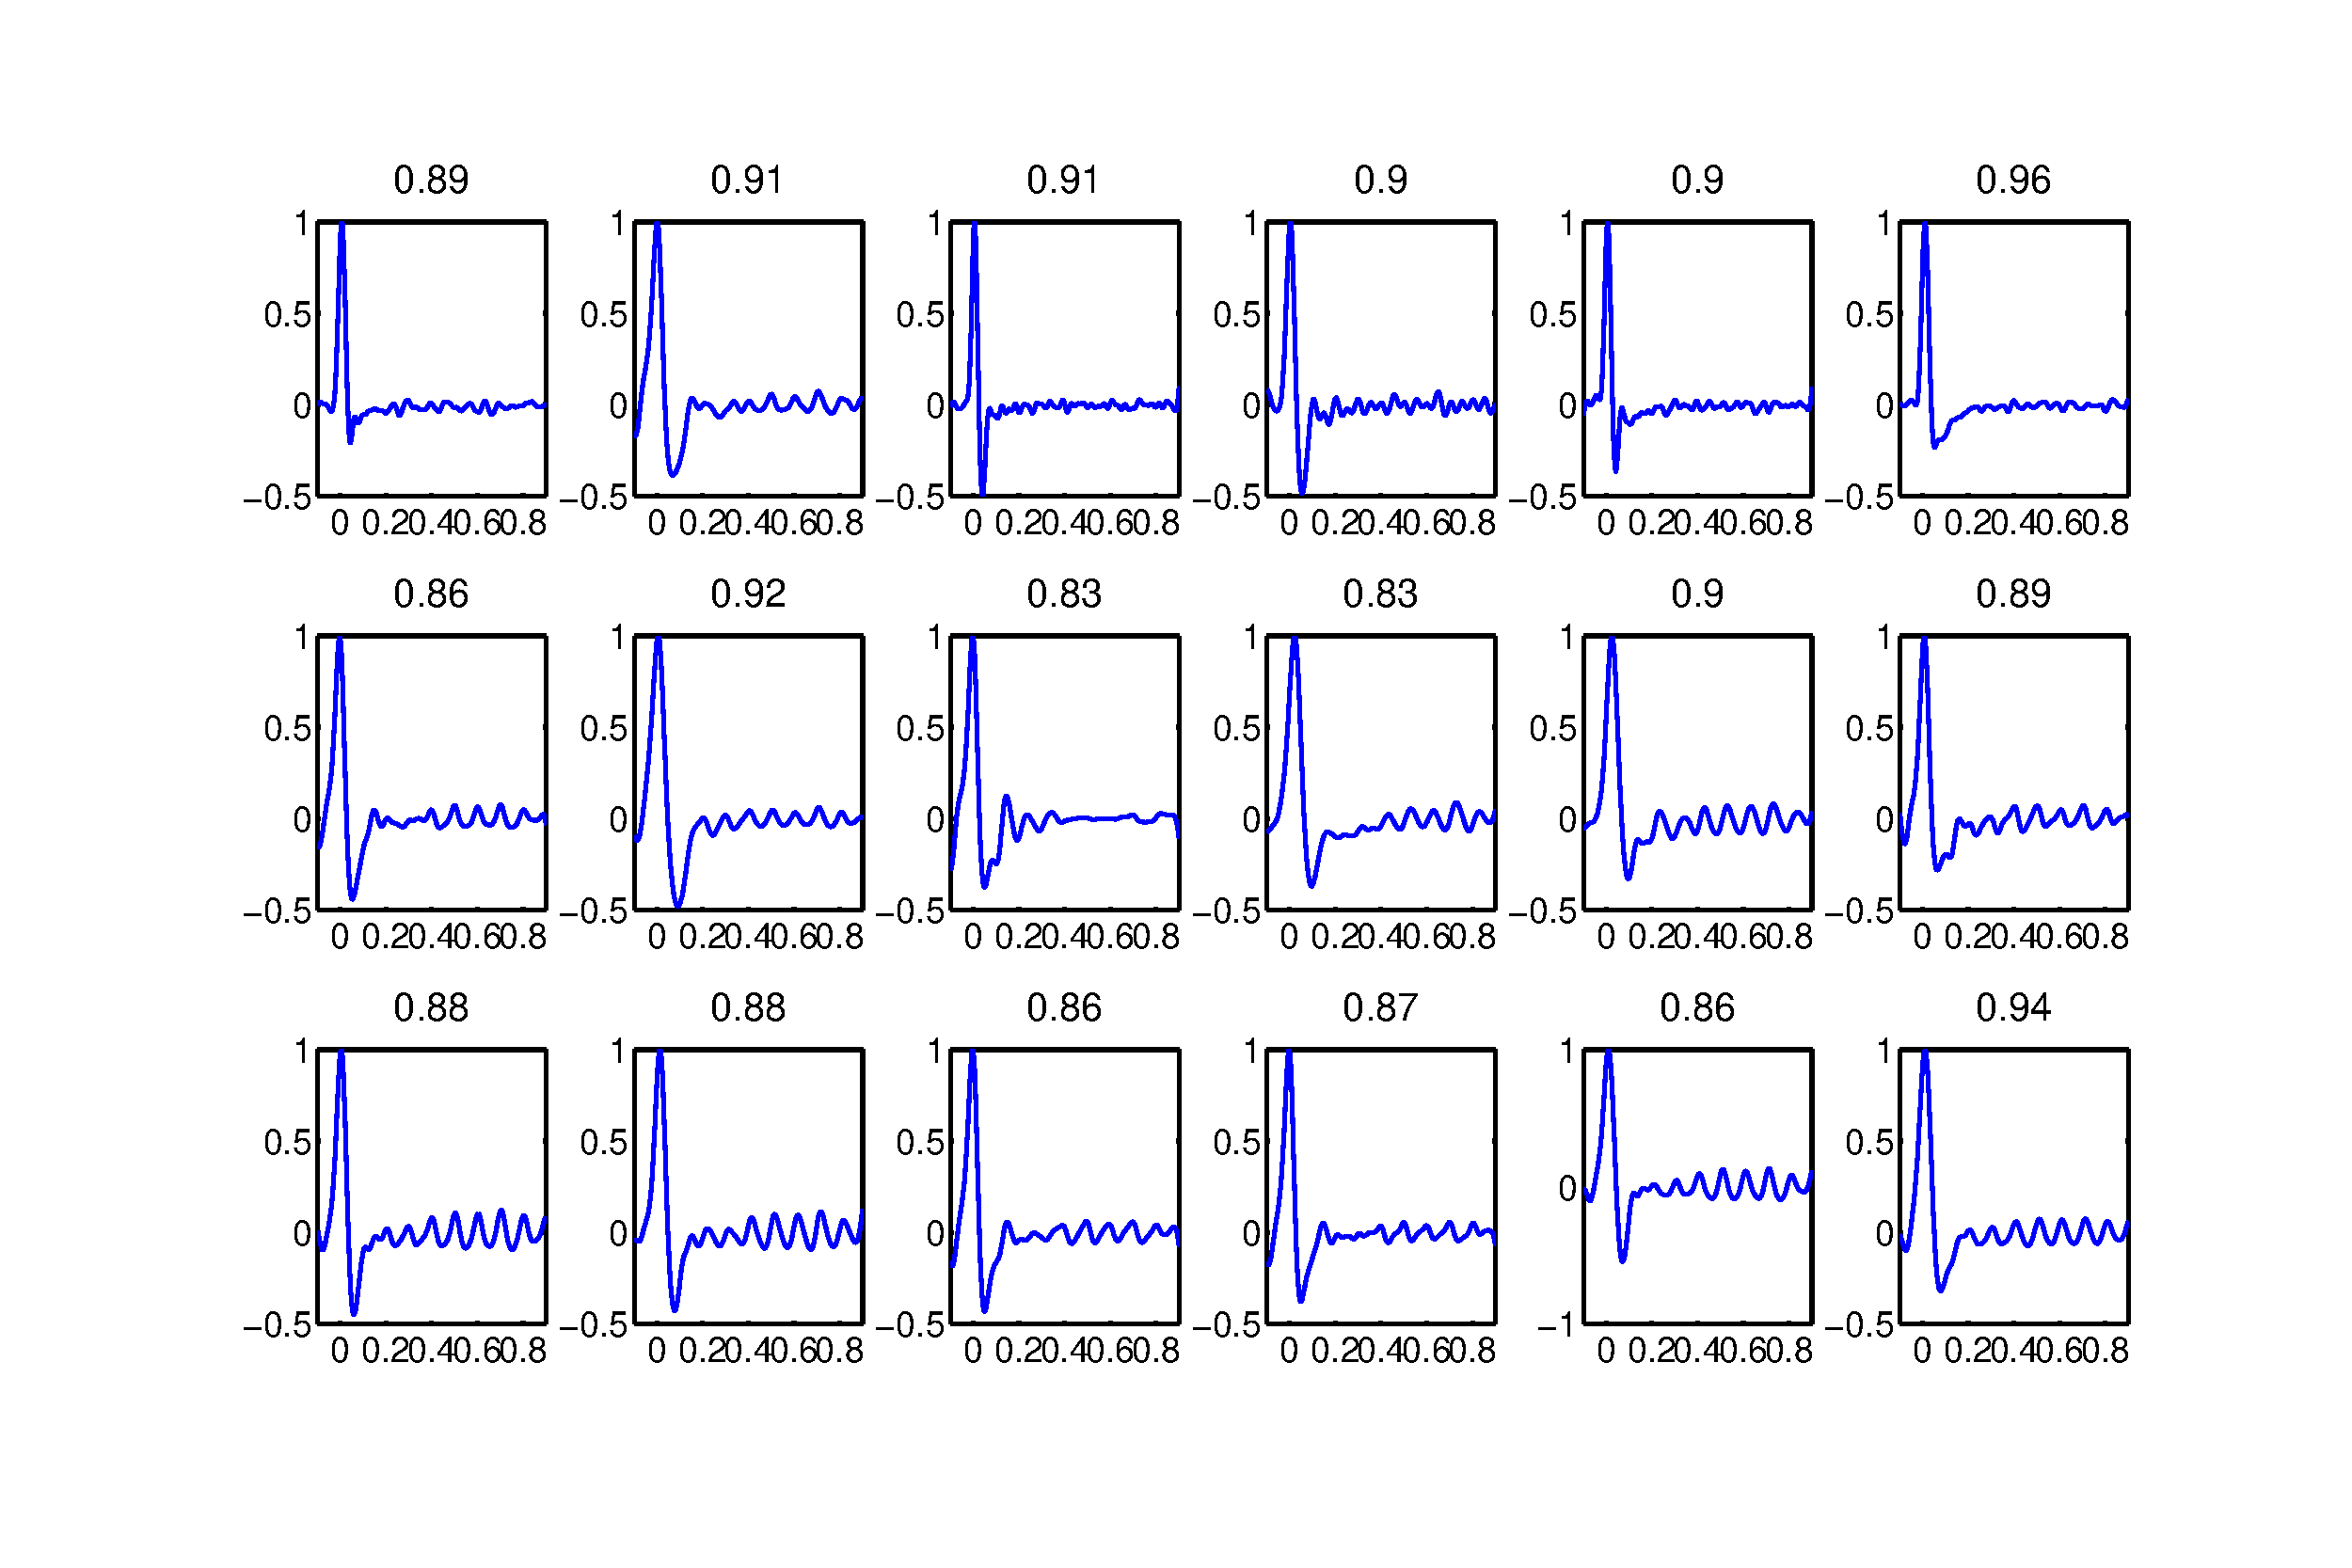
\includegraphics [width=\textwidth]{Analysis_February_01.pdf}
\begin{par}
The following figures show all the ORN responses and the predictions for each case overlaid in red. Notice that in most cases, the predicted firing rates are \ensuremath{<} 0 when the ORN stops firing.
\end{par} \vspace{1em}

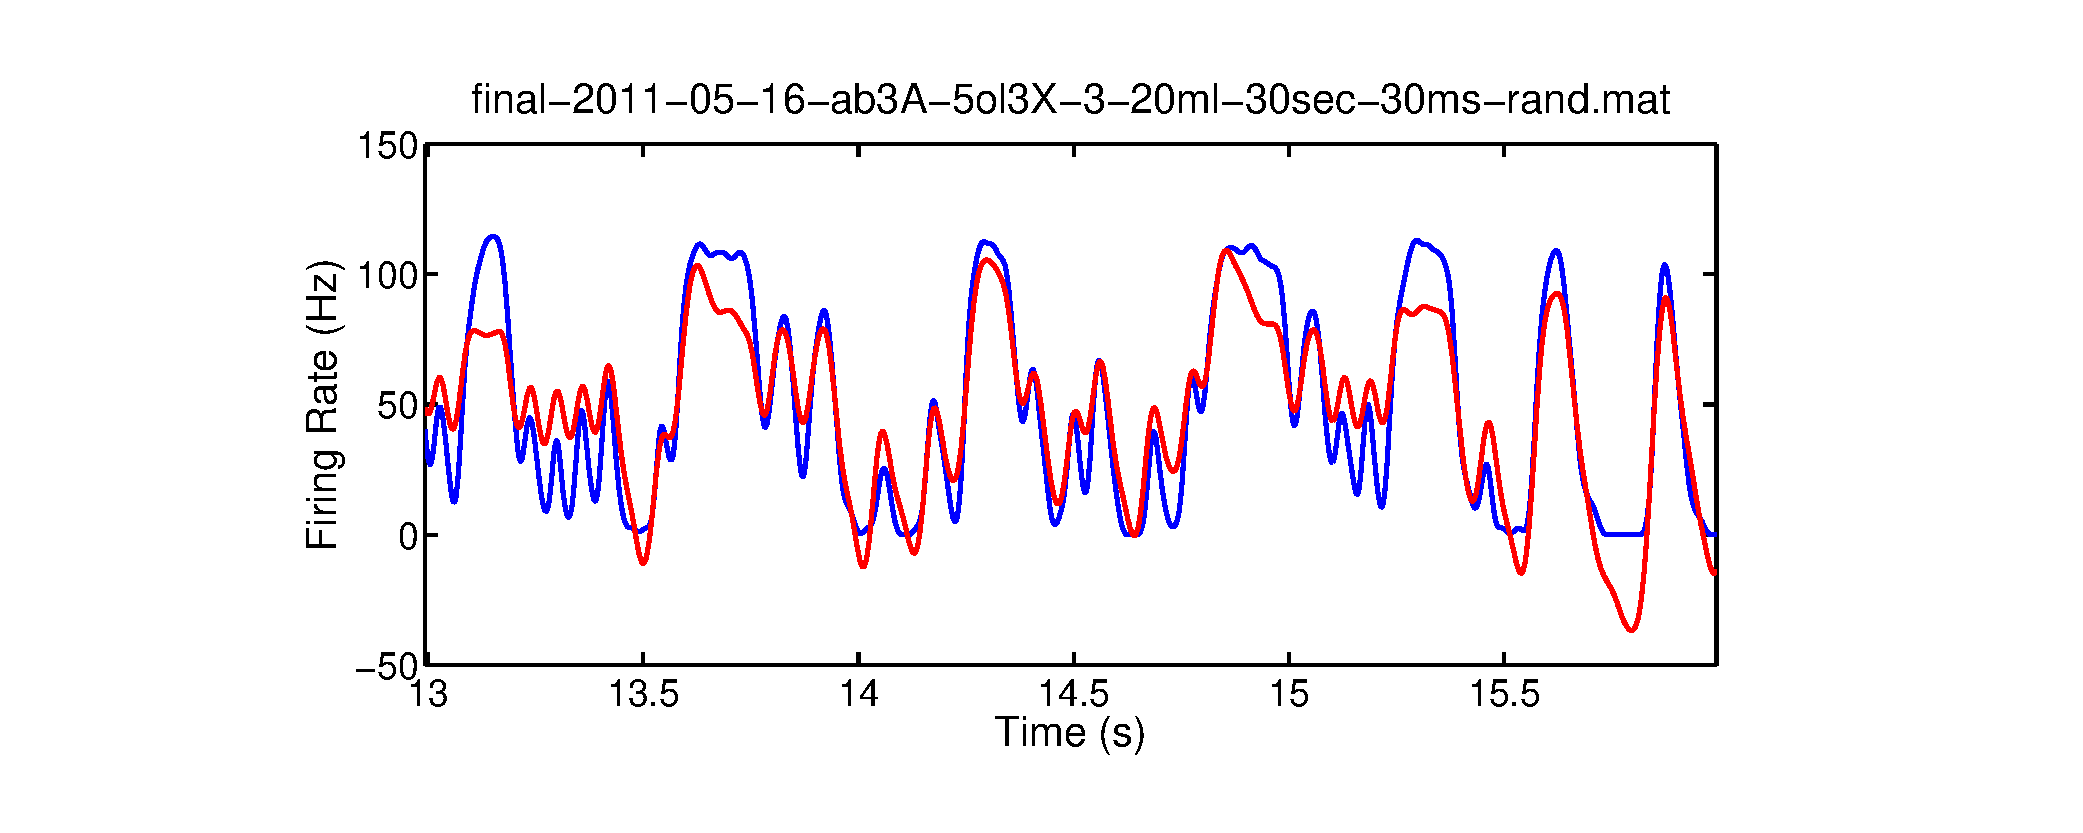
\includegraphics [width=\textwidth]{Analysis_February_02.pdf}

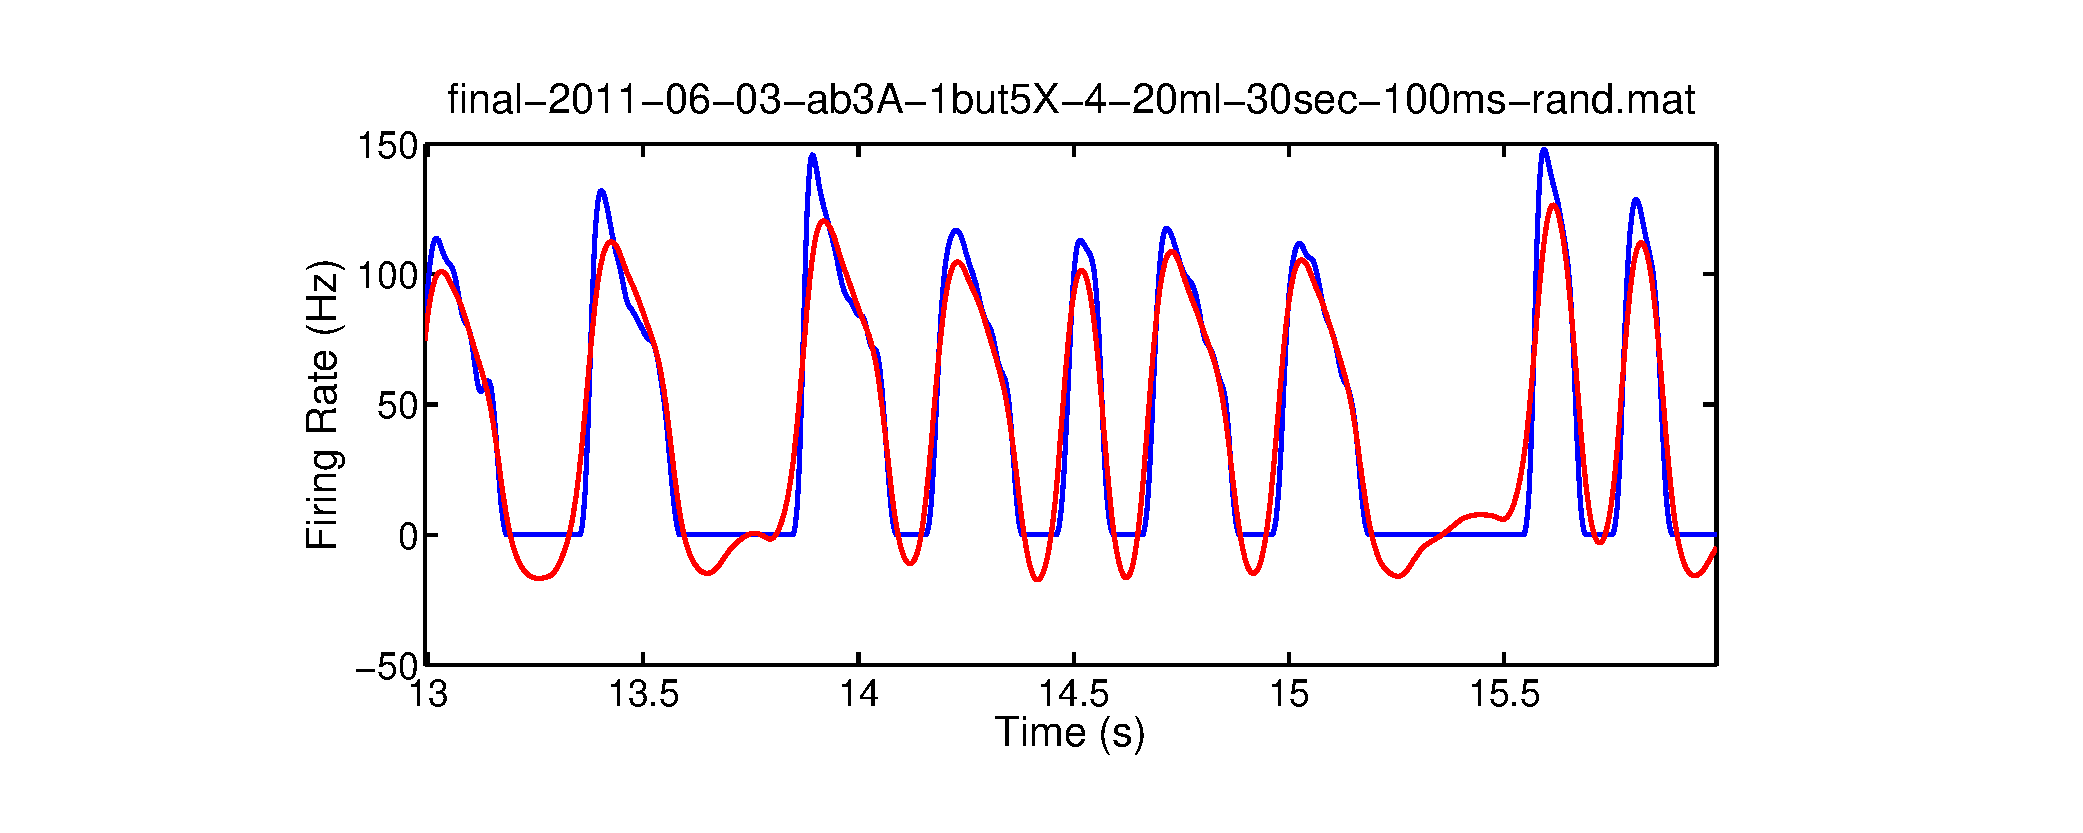
\includegraphics [width=\textwidth]{Analysis_February_03.pdf}

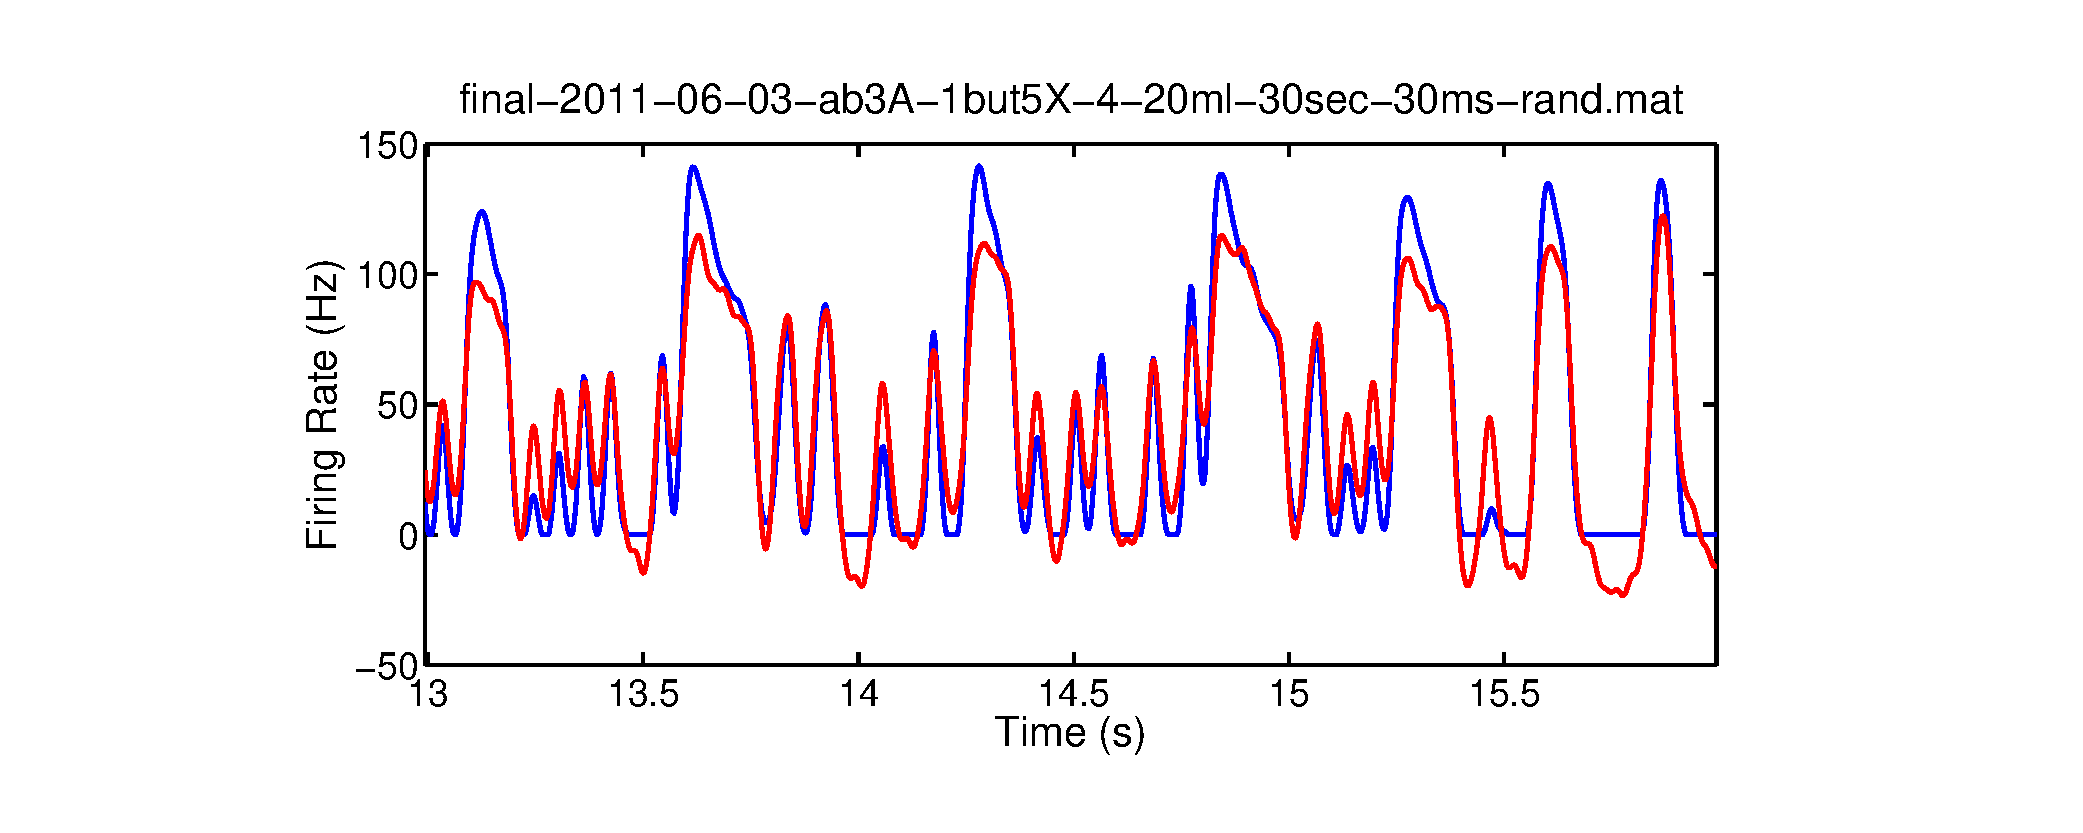
\includegraphics [width=\textwidth]{Analysis_February_04.pdf}

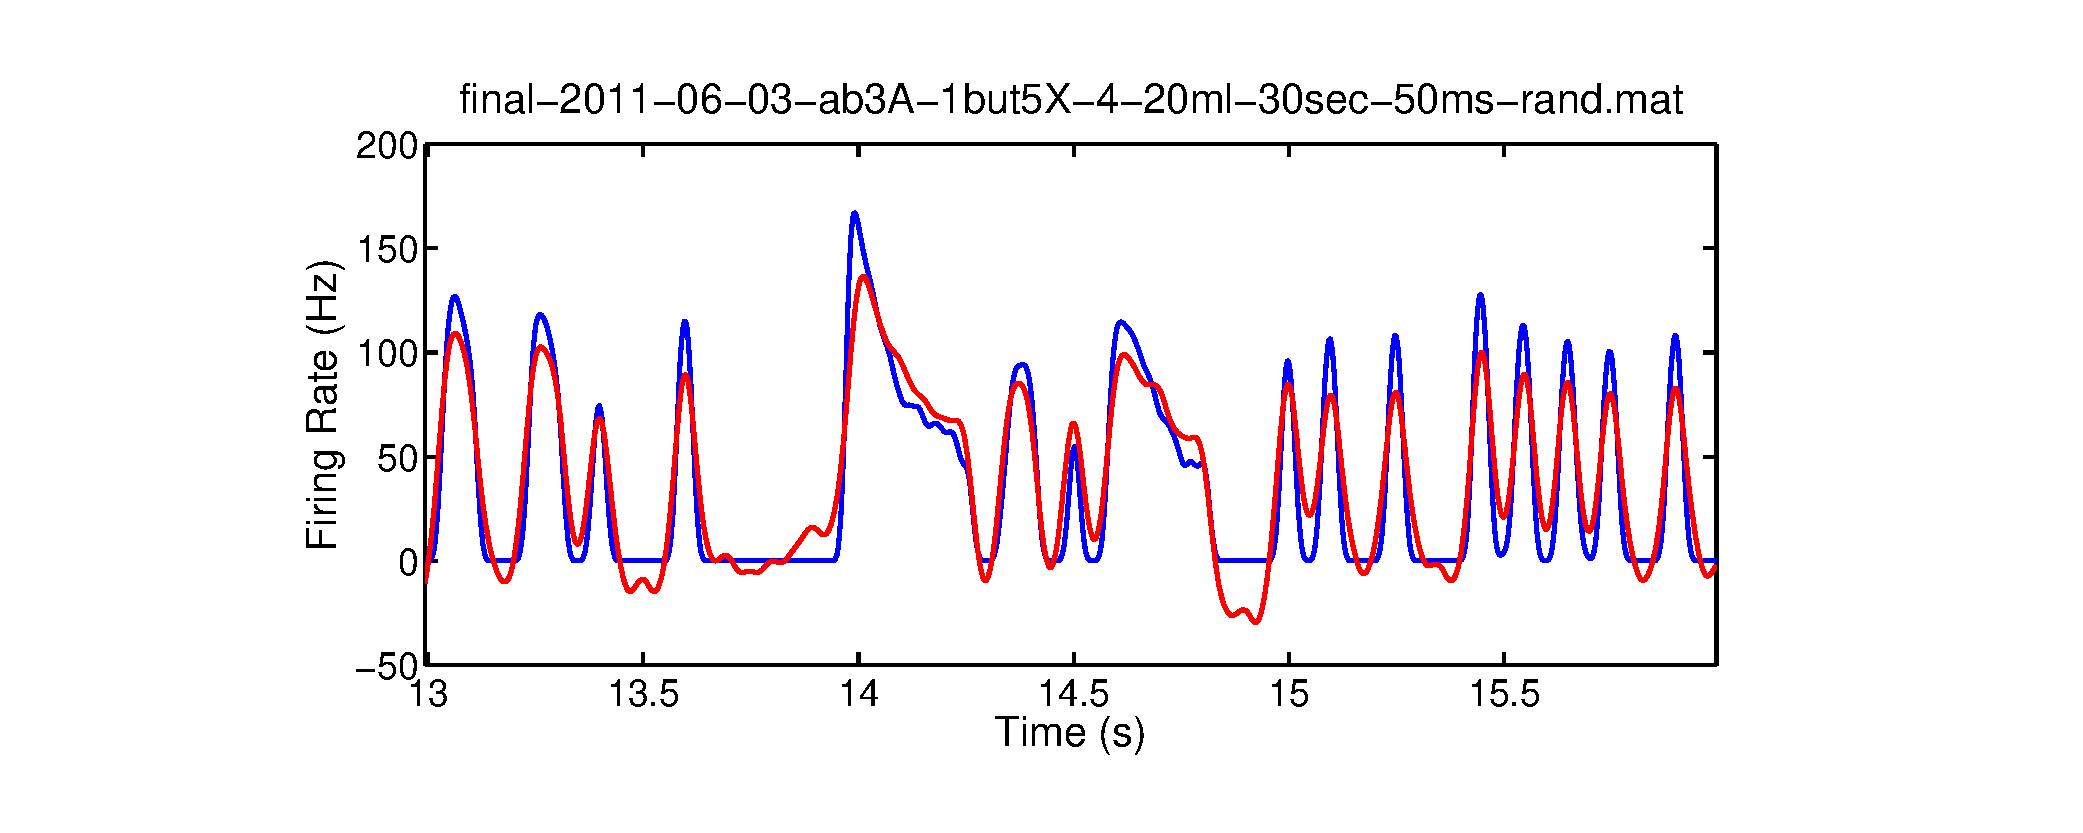
\includegraphics [width=\textwidth]{Analysis_February_05.pdf}

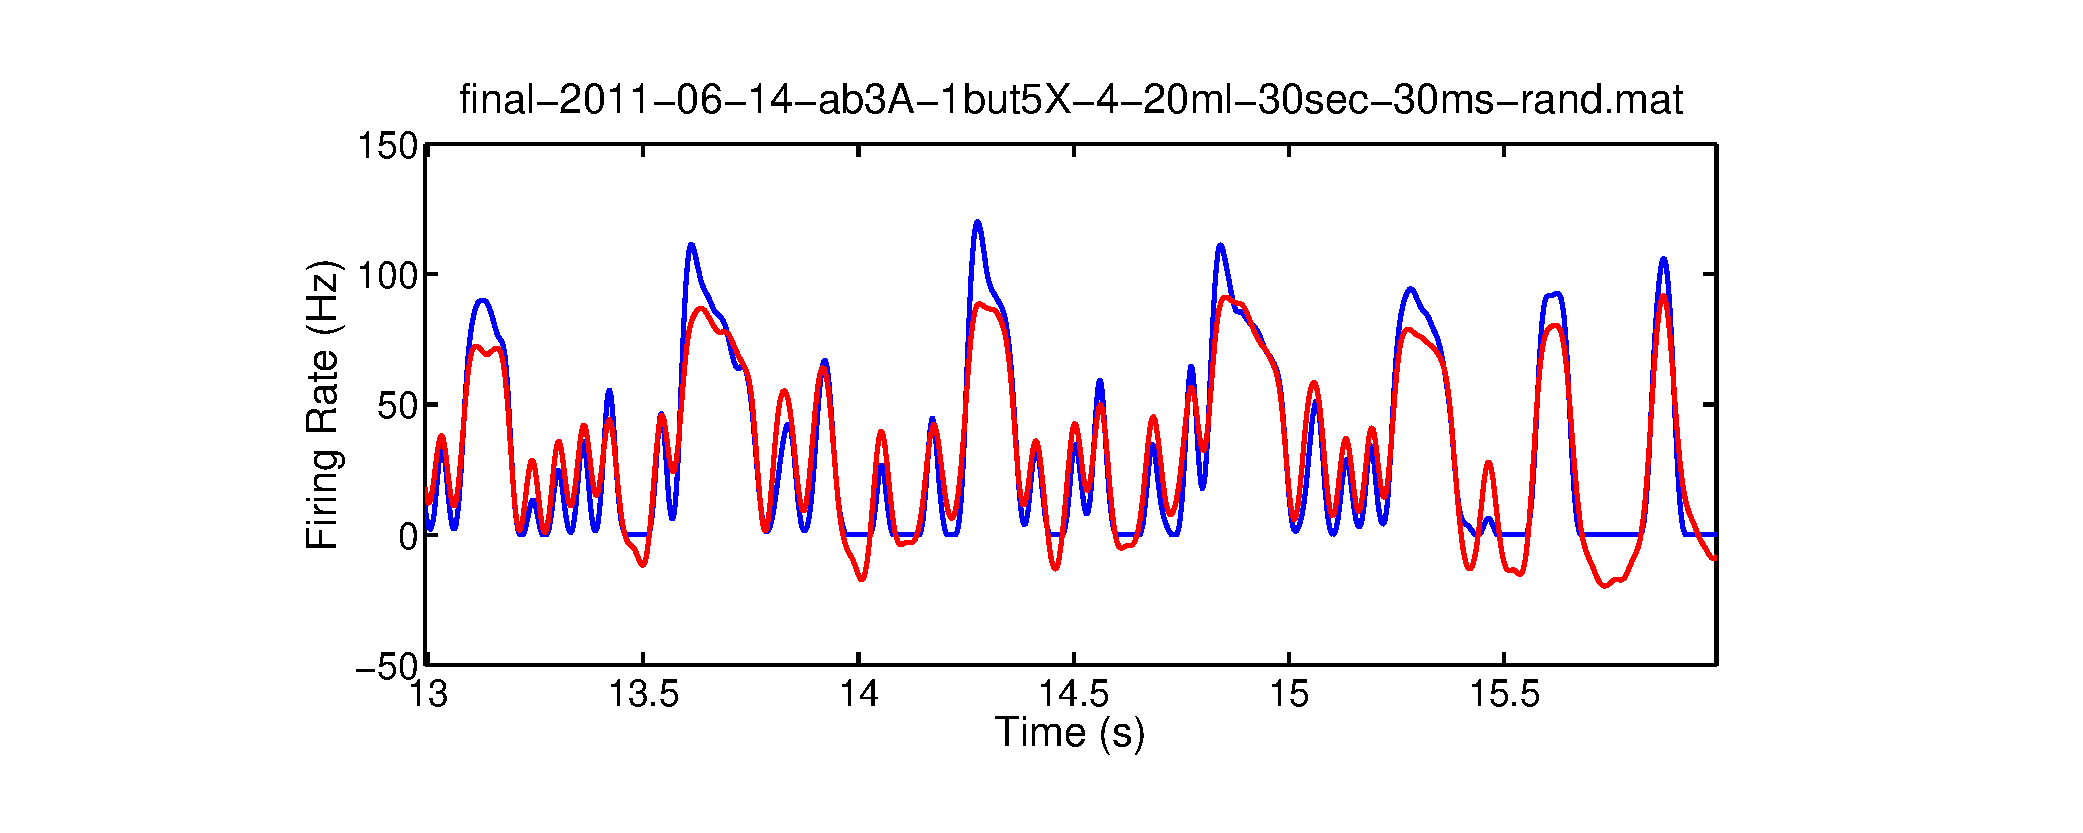
\includegraphics [width=\textwidth]{Analysis_February_06.pdf}

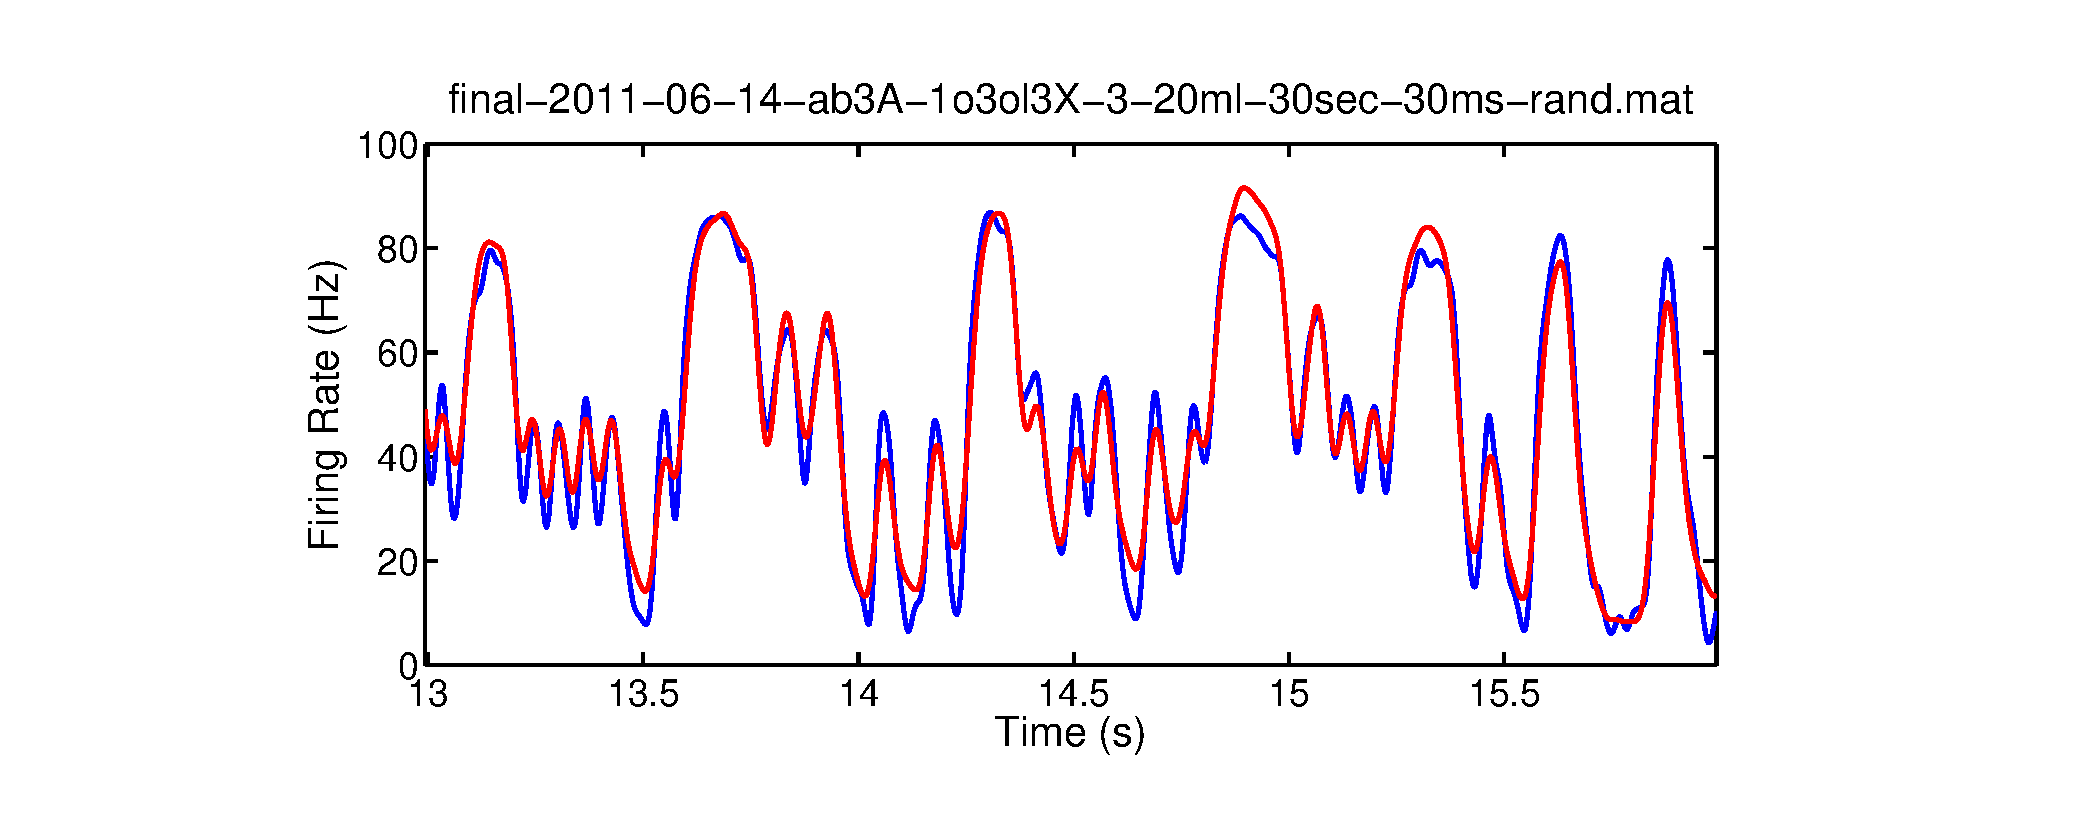
\includegraphics [width=\textwidth]{Analysis_February_07.pdf}

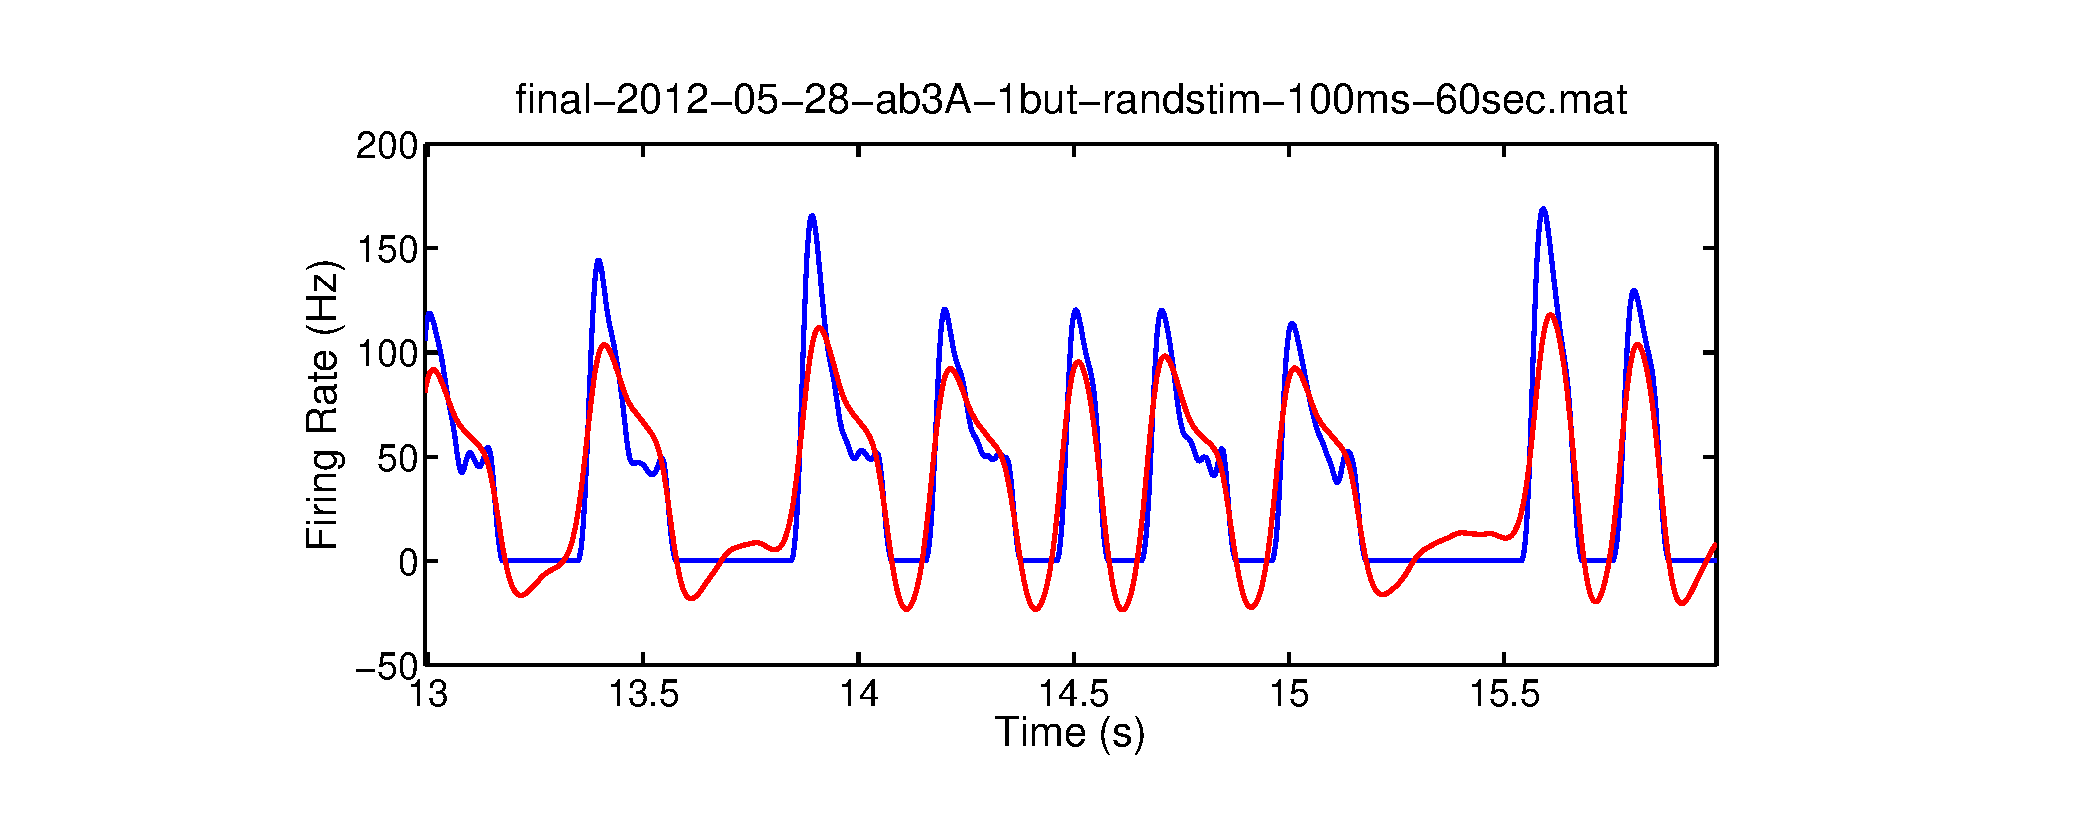
\includegraphics [width=\textwidth]{Analysis_February_08.pdf}

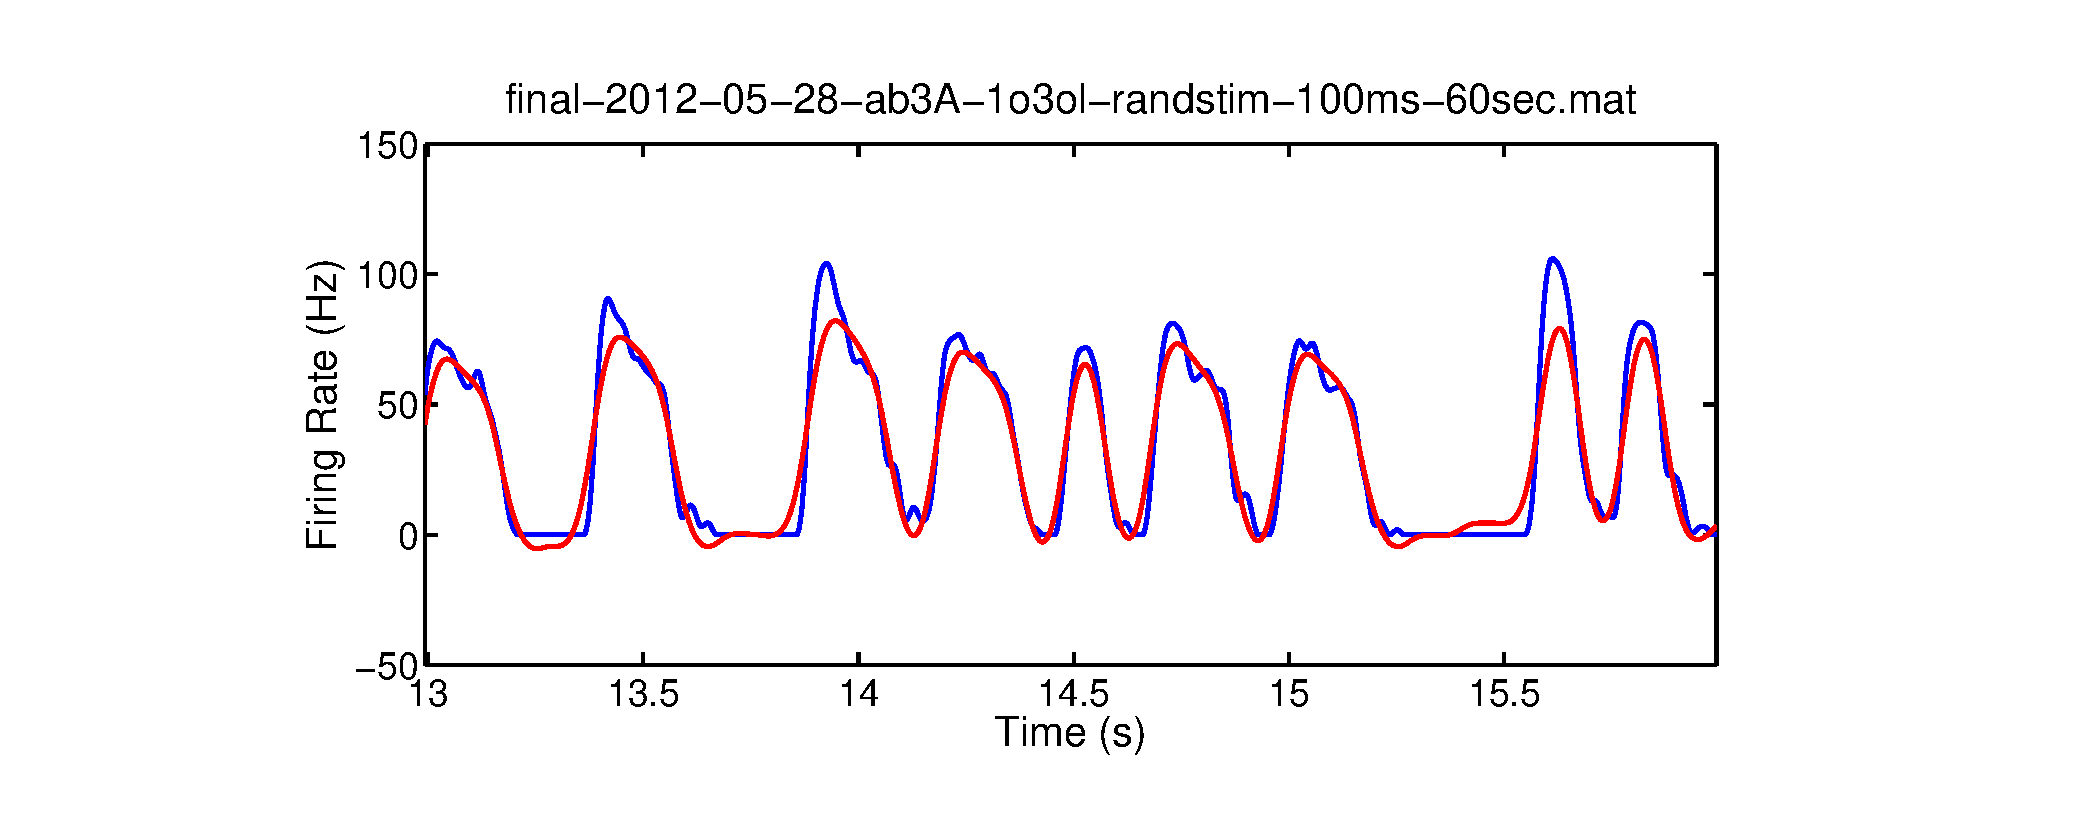
\includegraphics [width=\textwidth]{Analysis_February_09.pdf}

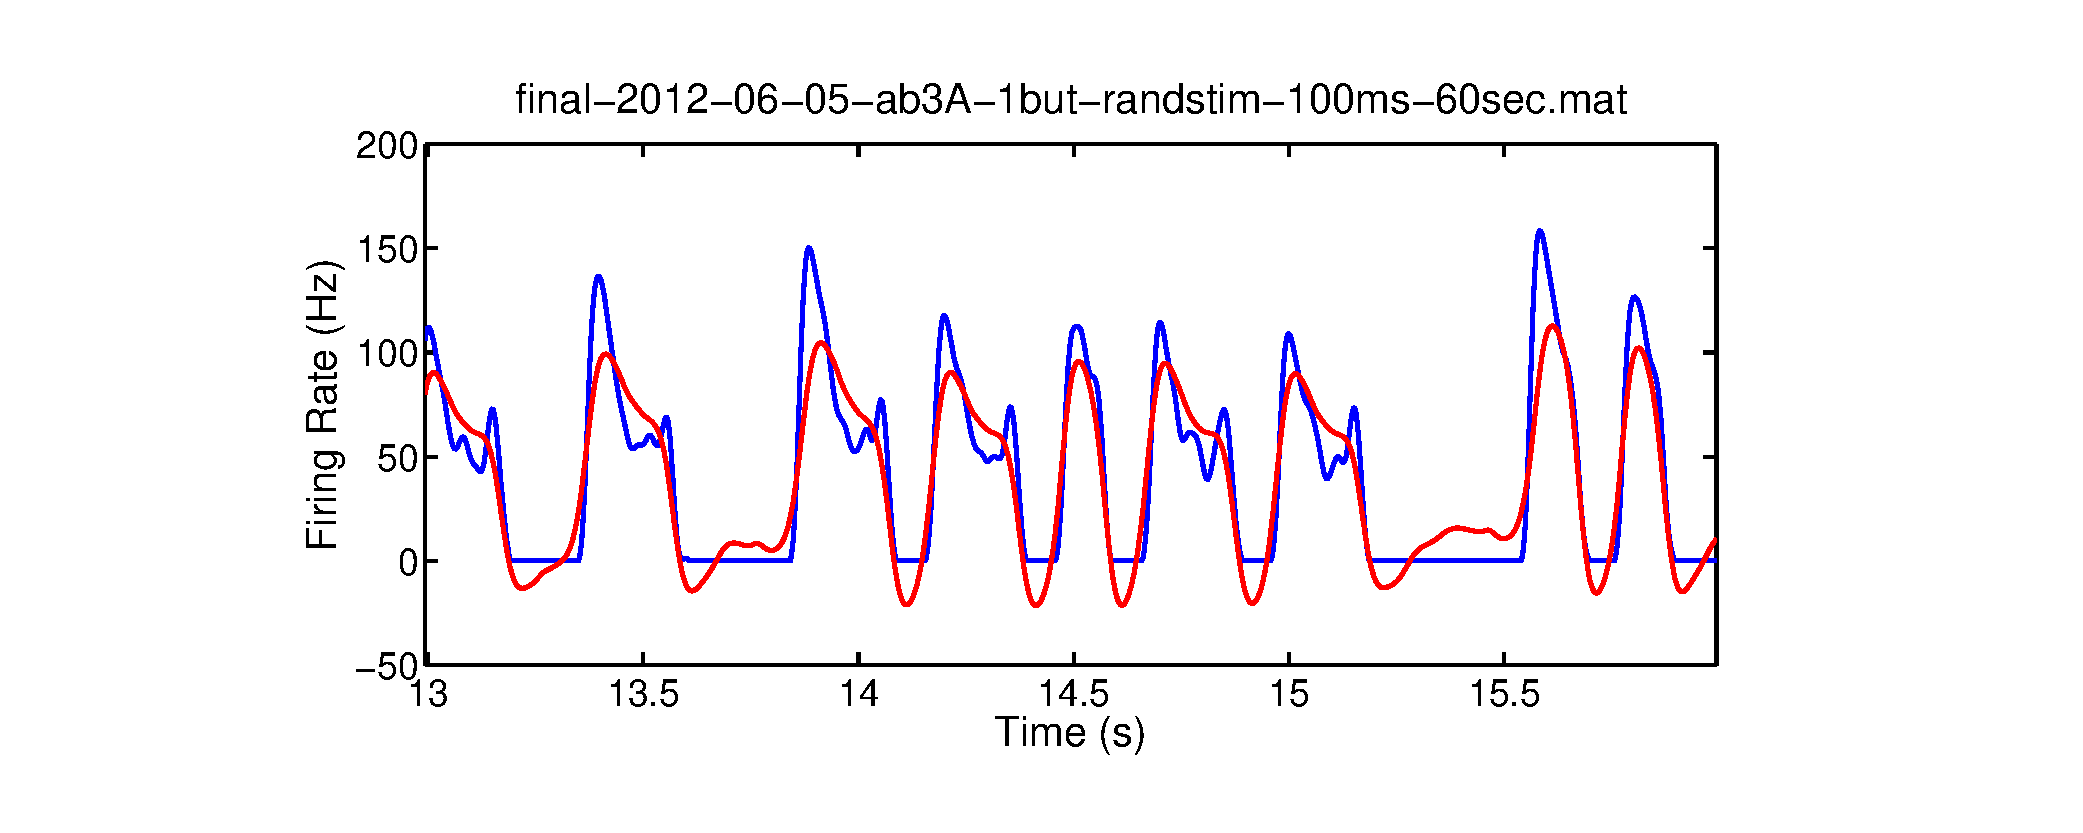
\includegraphics [width=\textwidth]{Analysis_February_10.pdf}

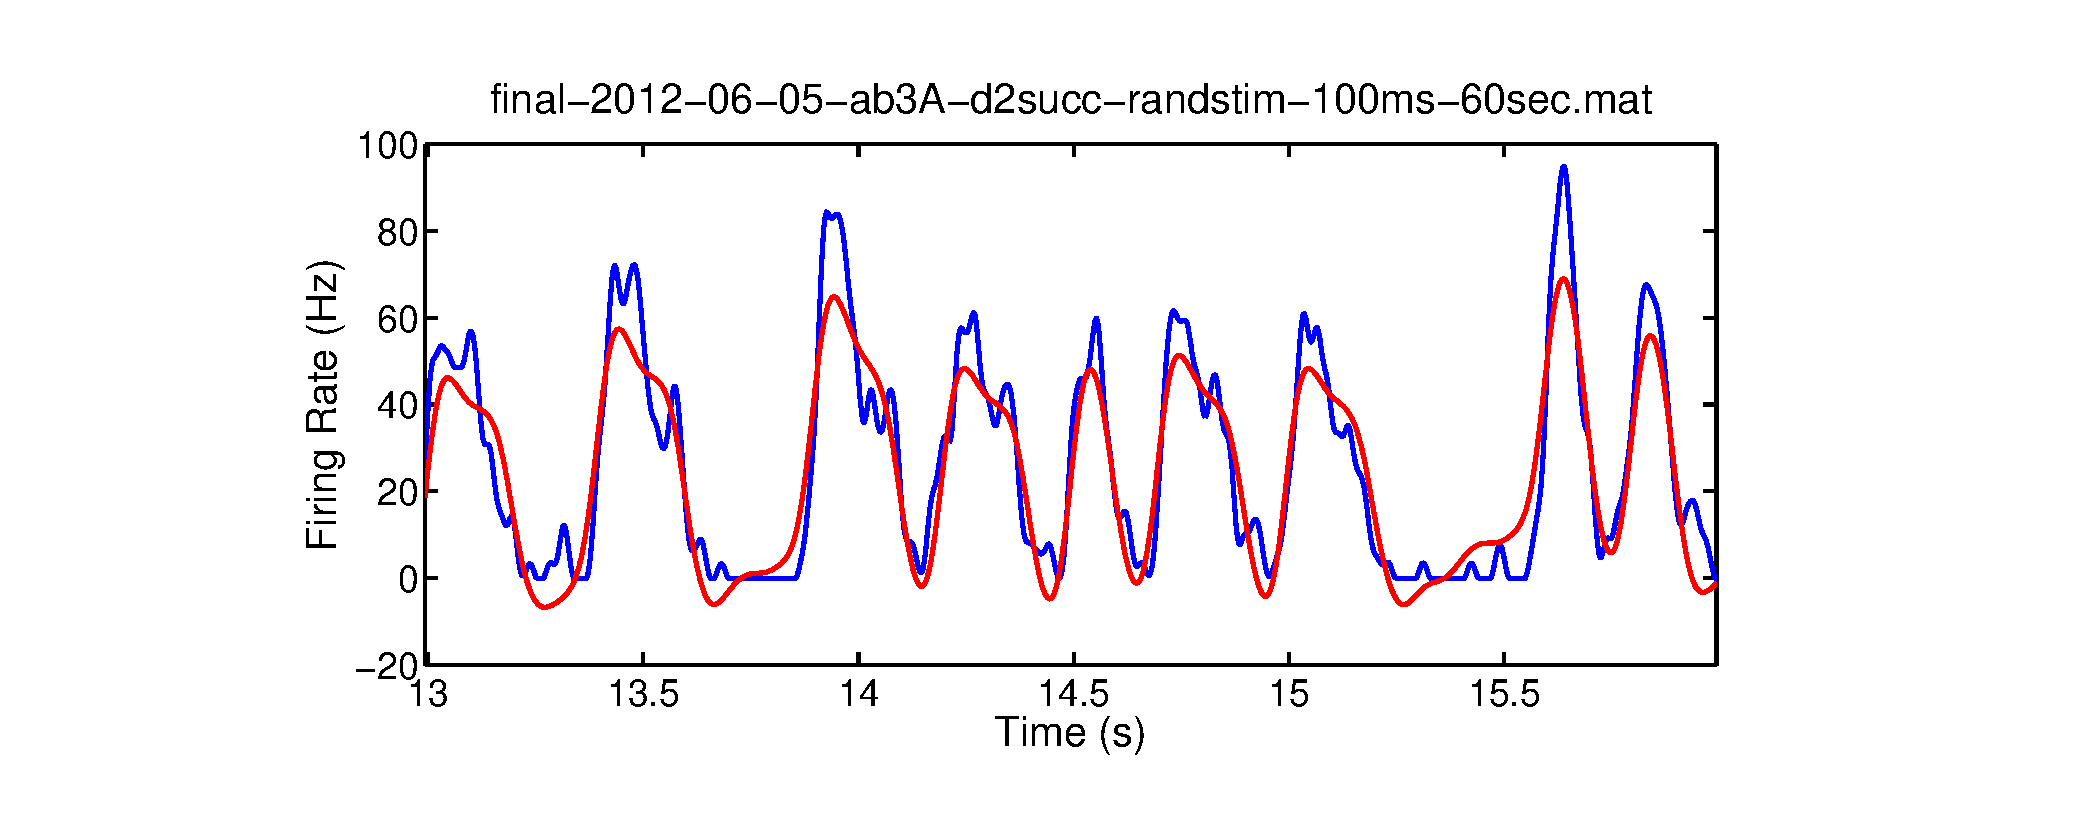
\includegraphics [width=\textwidth]{Analysis_February_11.pdf}

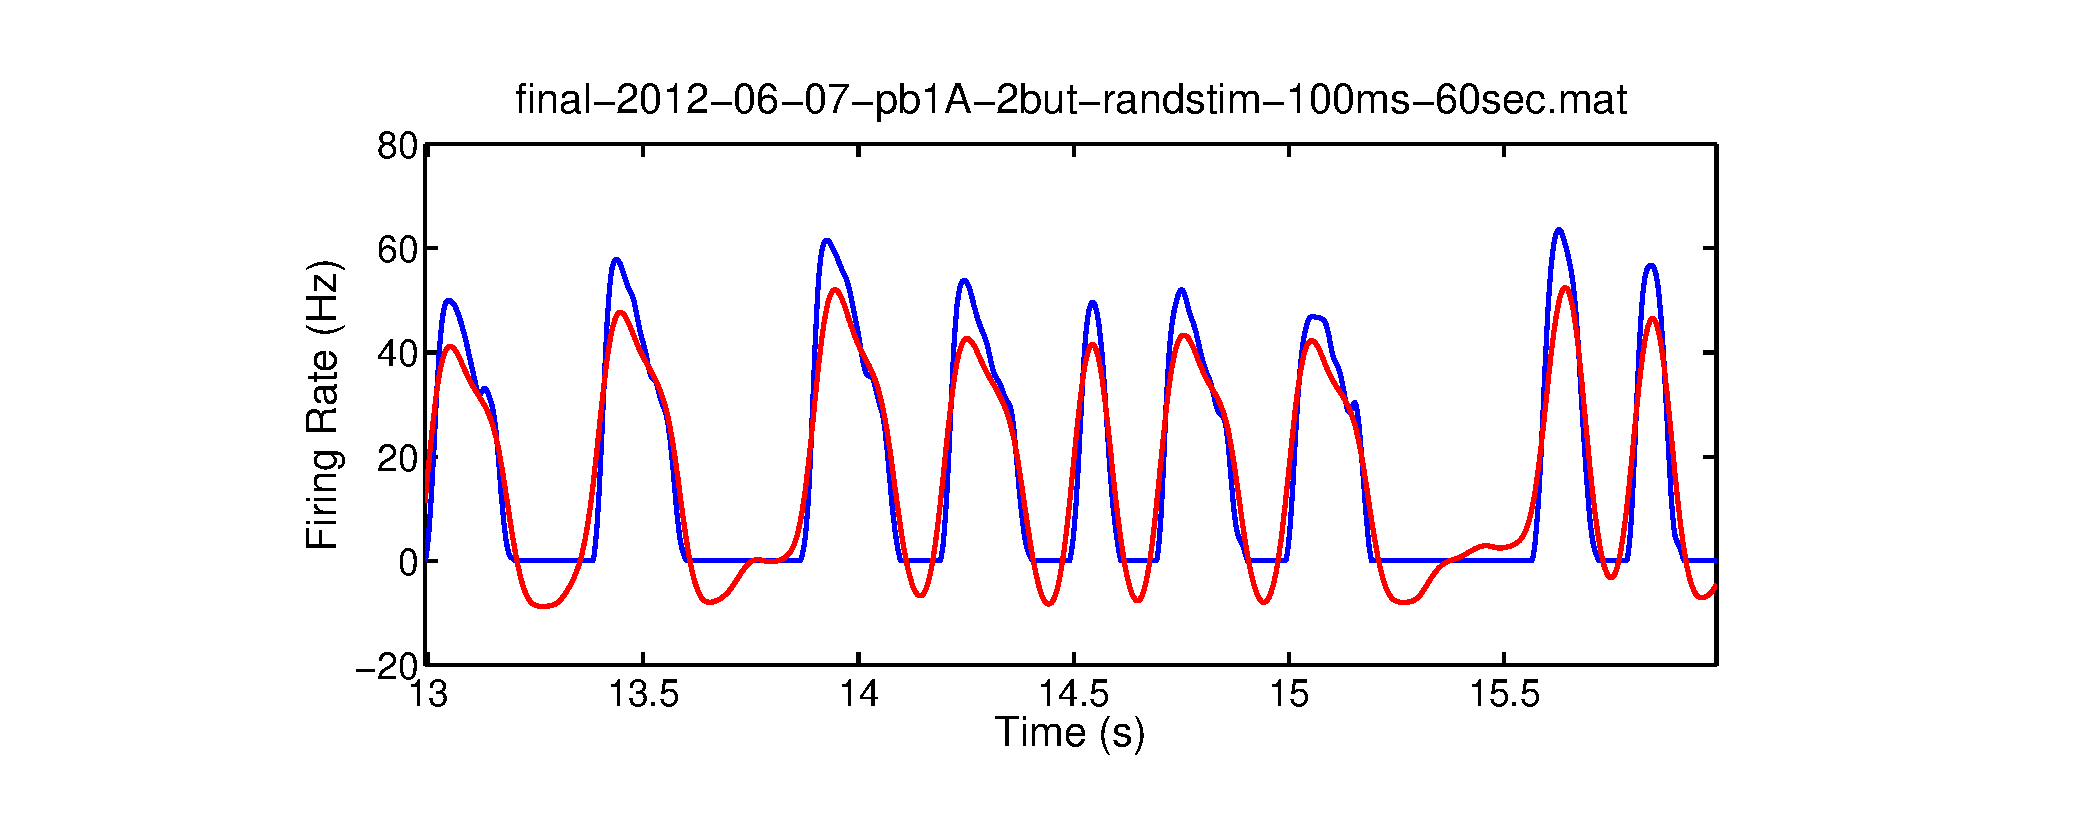
\includegraphics [width=\textwidth]{Analysis_February_12.pdf}

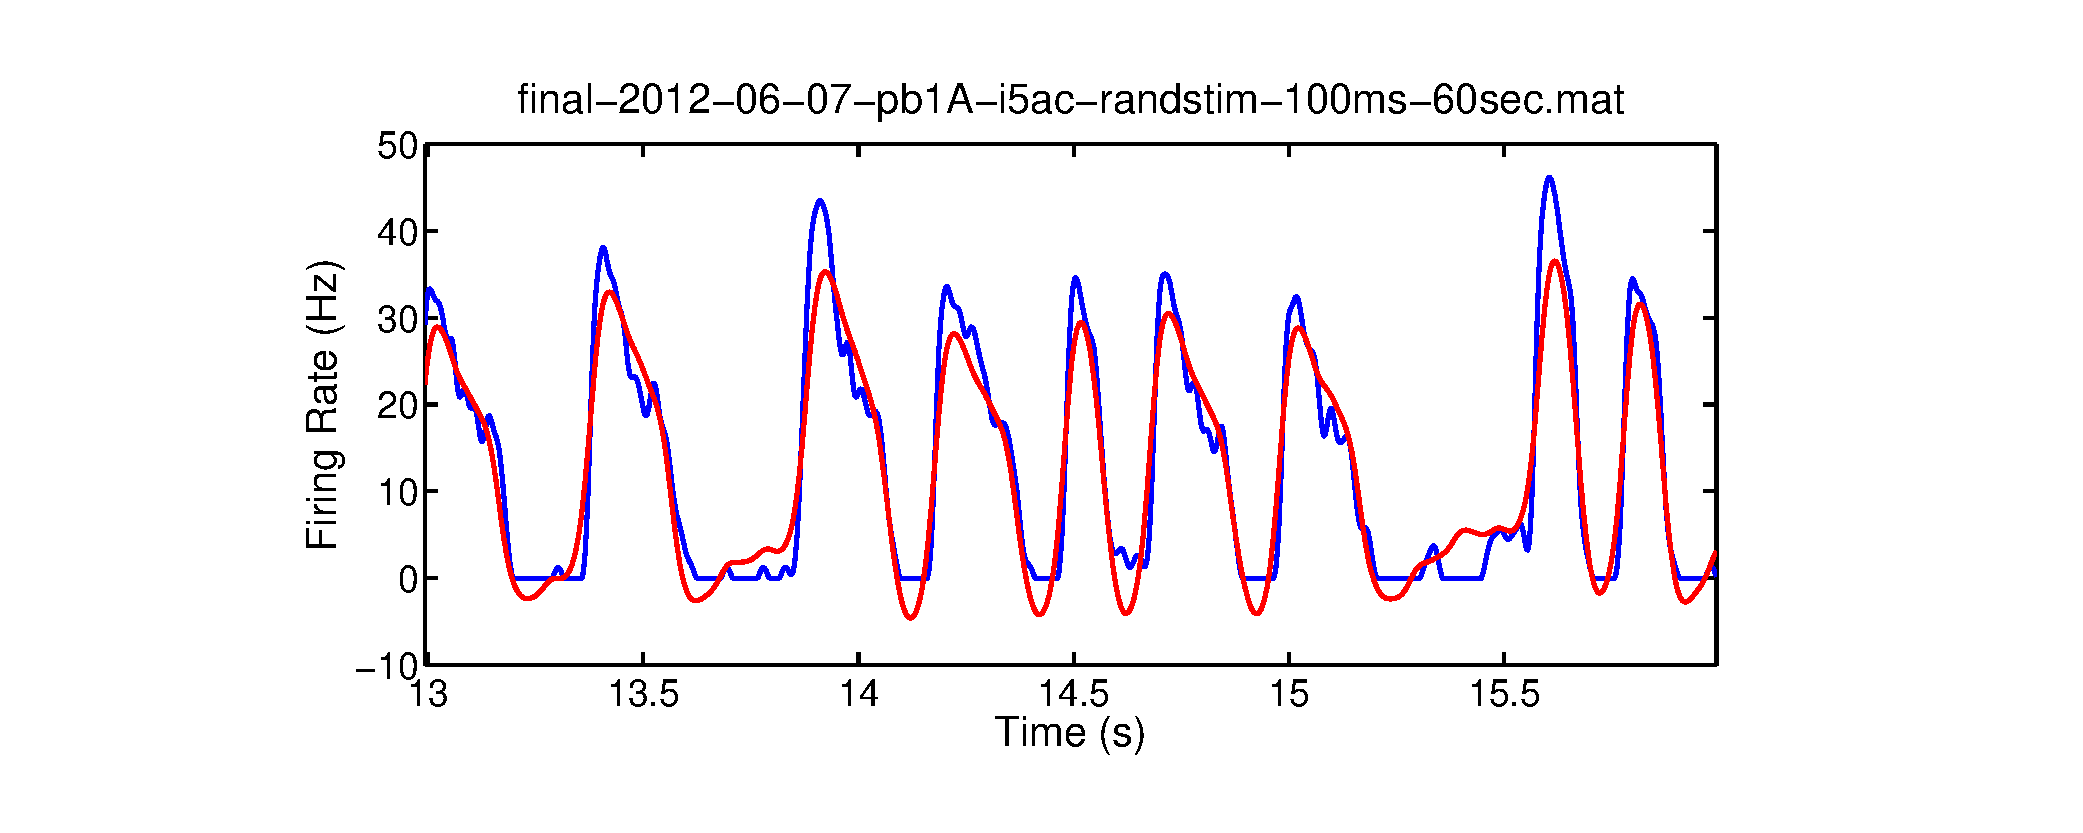
\includegraphics [width=\textwidth]{Analysis_February_13.pdf}

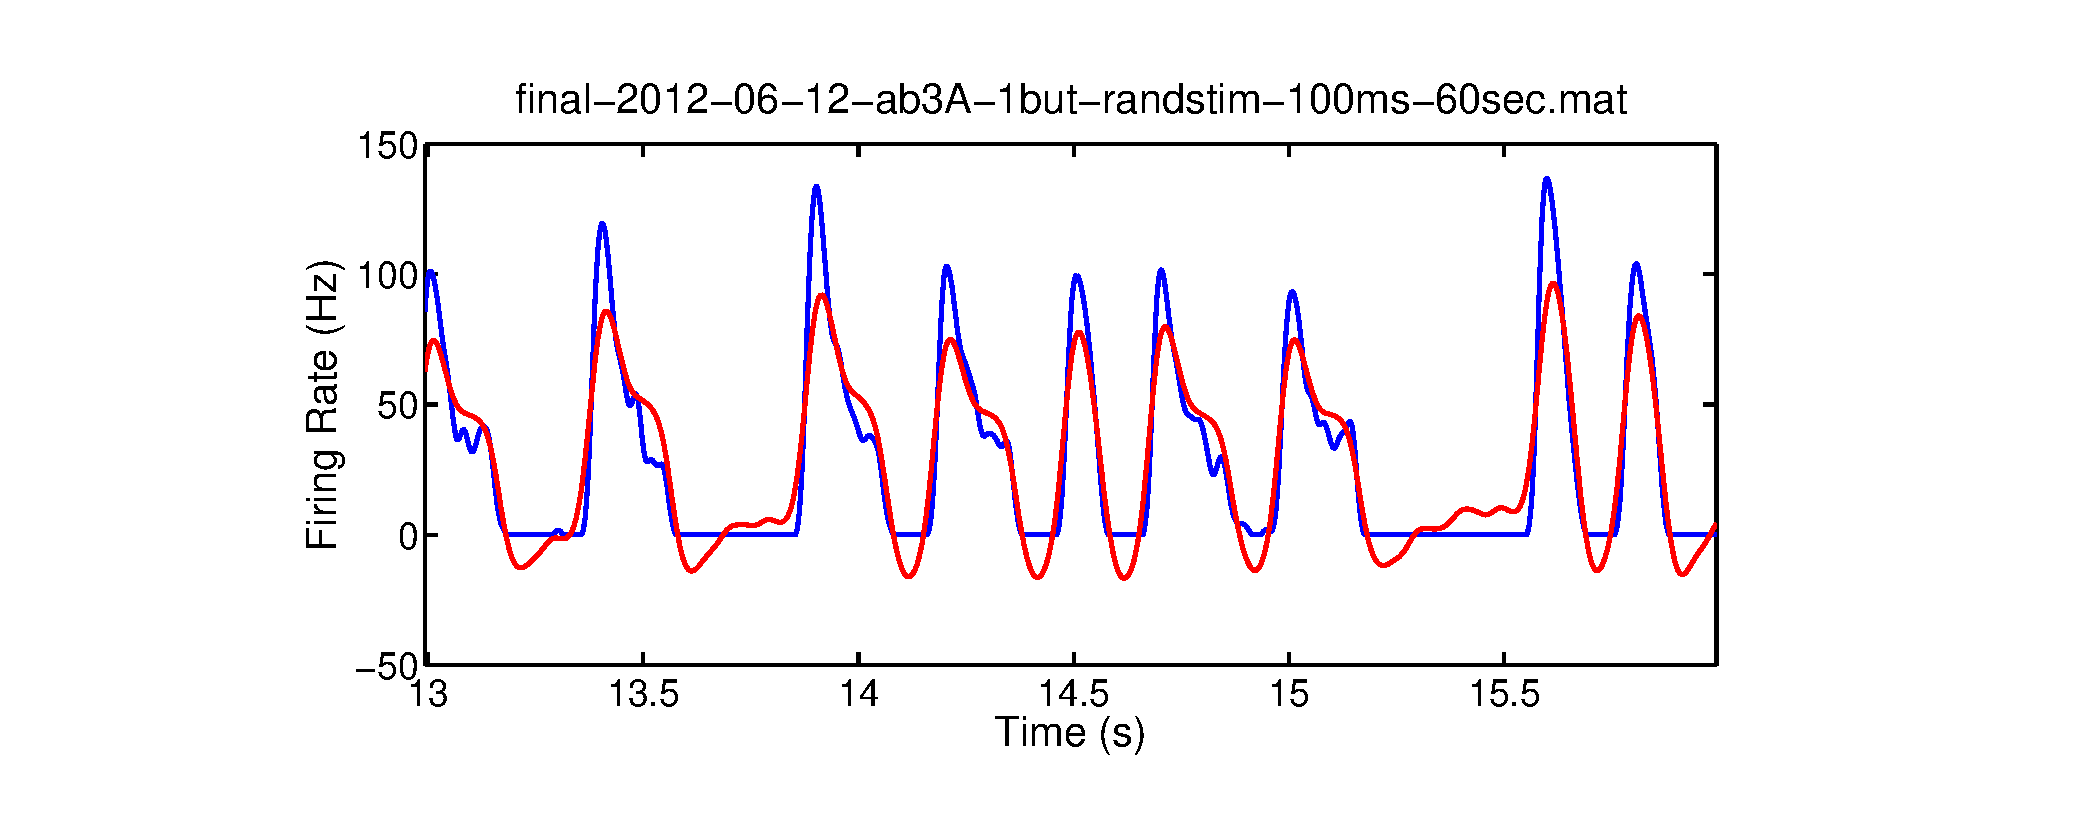
\includegraphics [width=\textwidth]{Analysis_February_14.pdf}

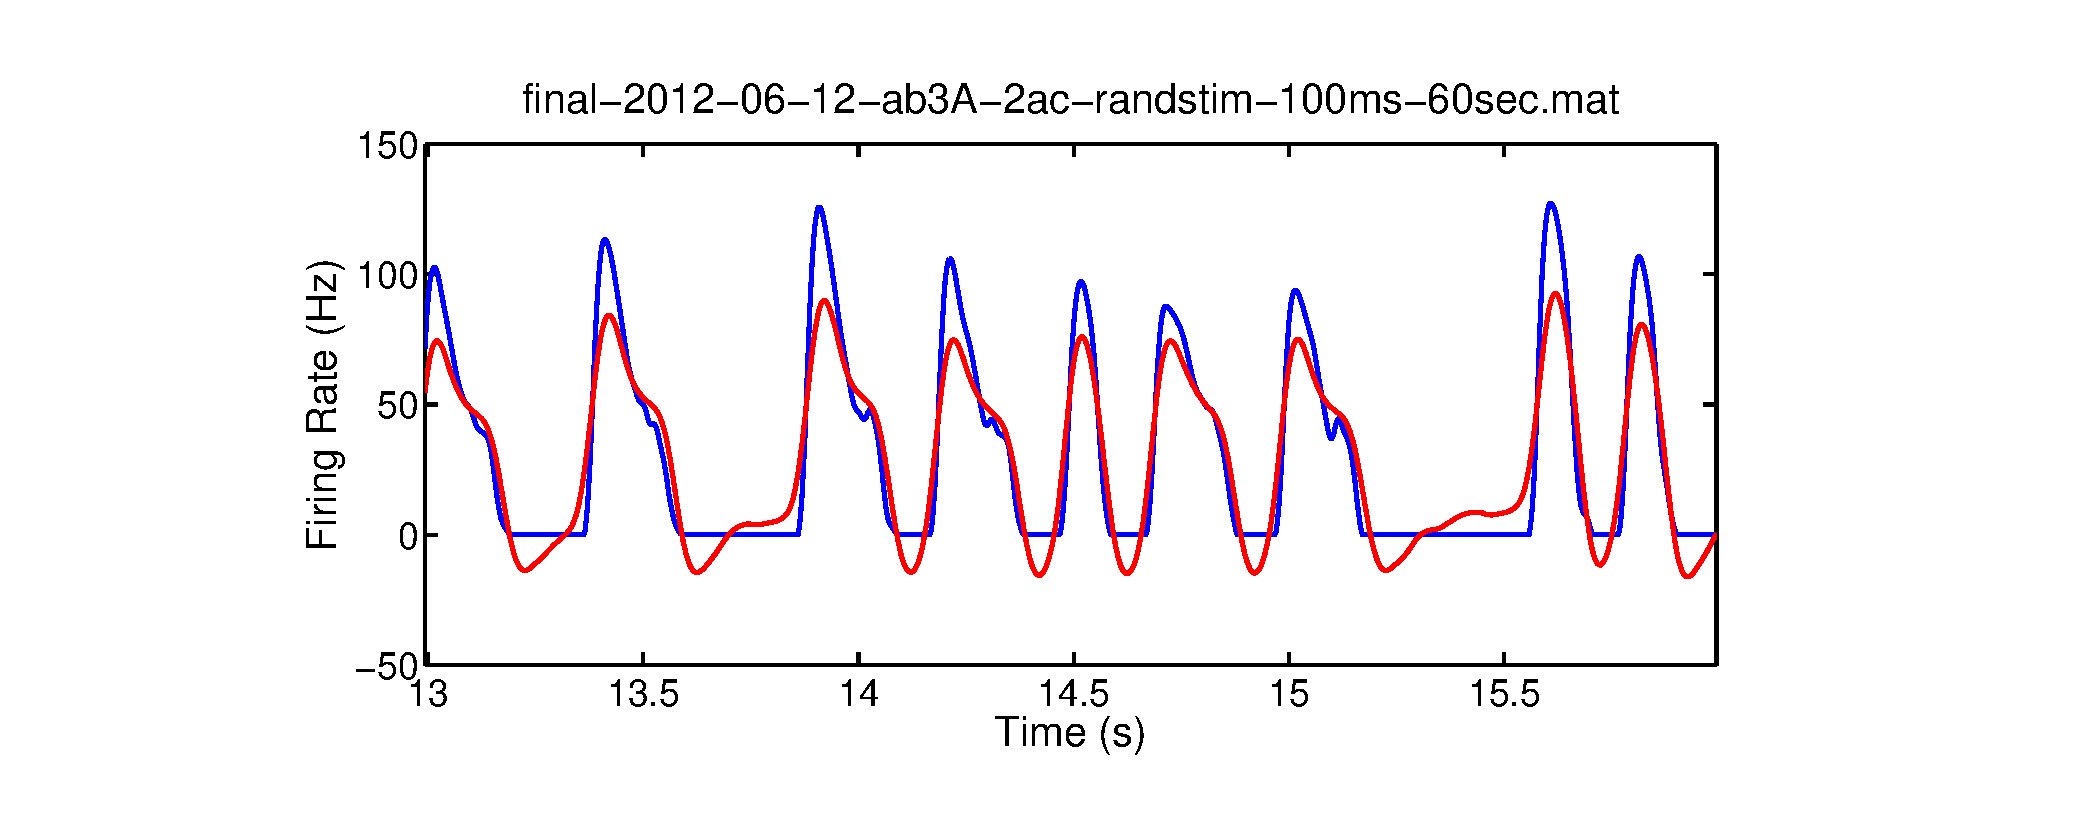
\includegraphics [width=\textwidth]{Analysis_February_15.pdf}

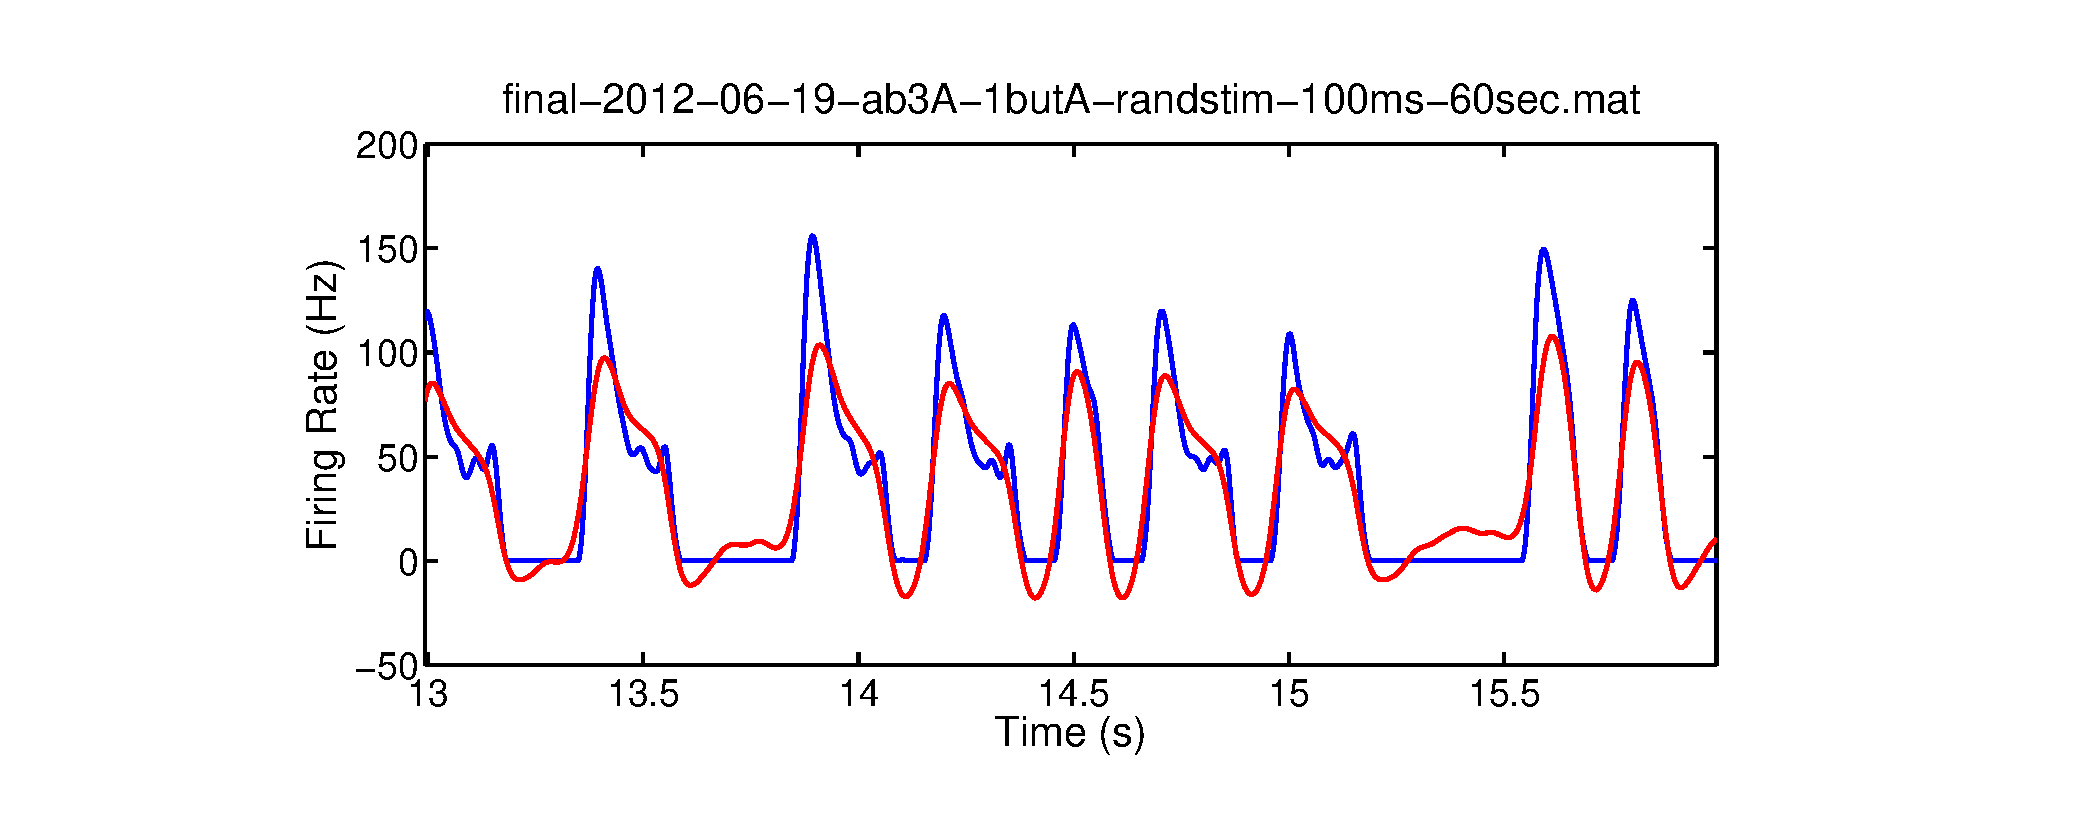
\includegraphics [width=\textwidth]{Analysis_February_16.pdf}

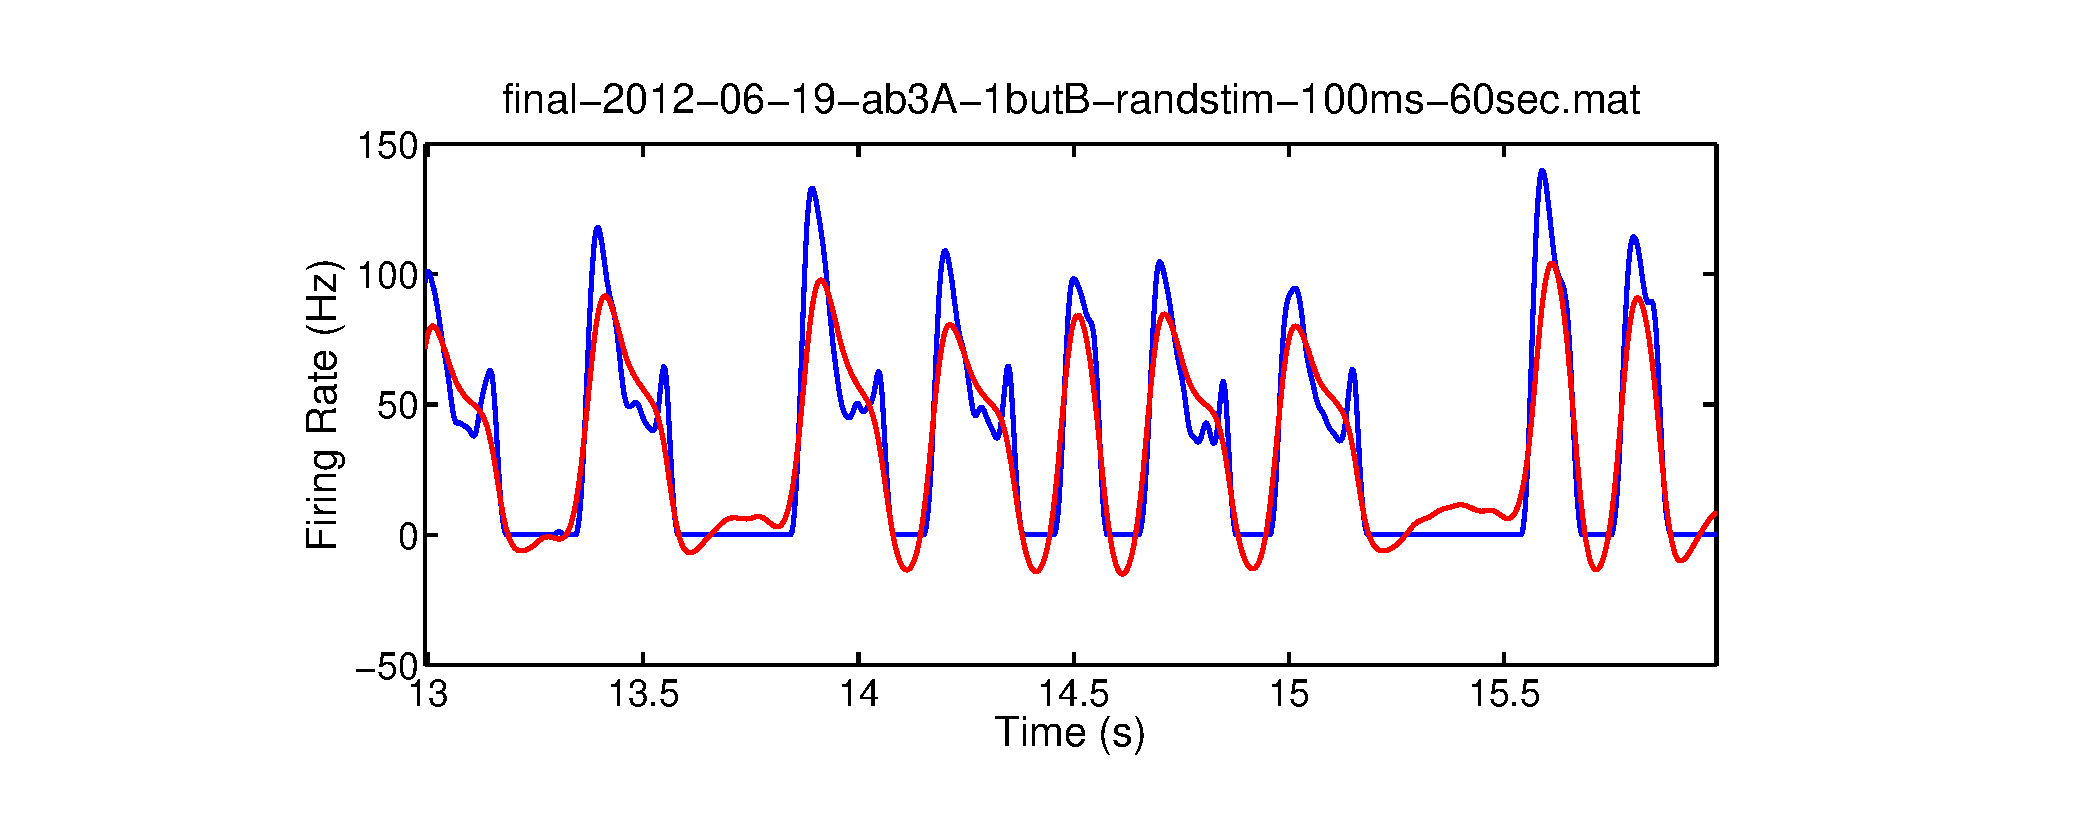
\includegraphics [width=\textwidth]{Analysis_February_17.pdf}

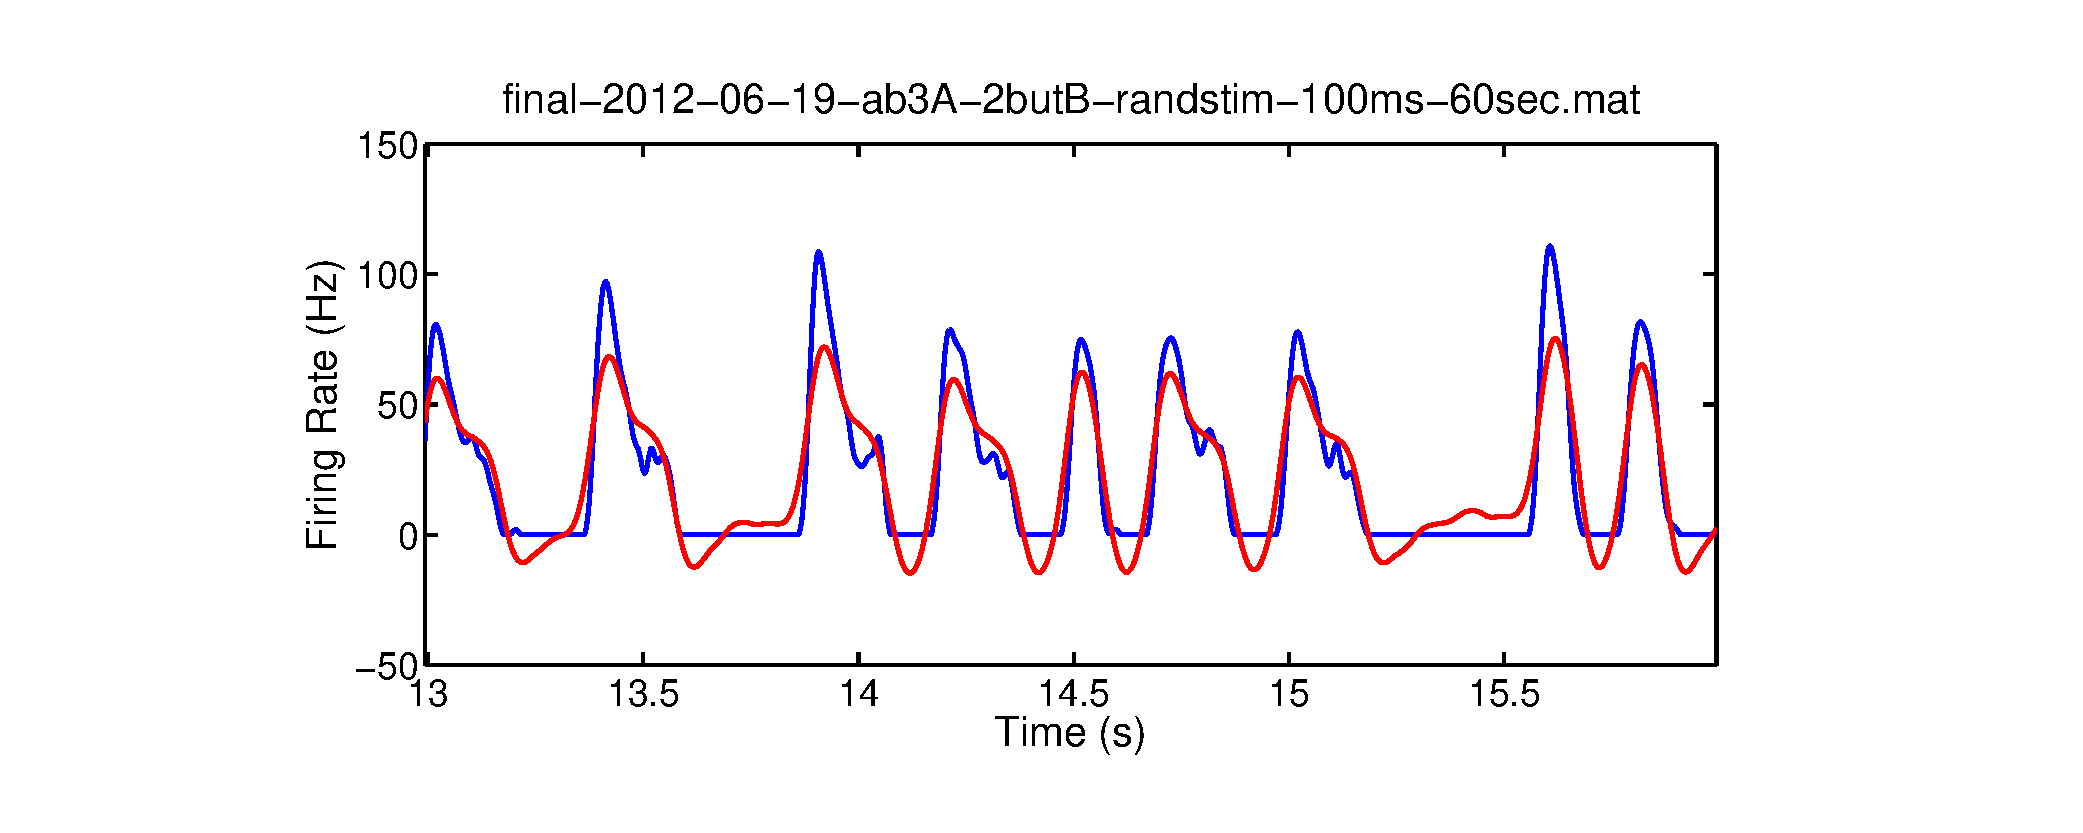
\includegraphics [width=\textwidth]{Analysis_February_18.pdf}

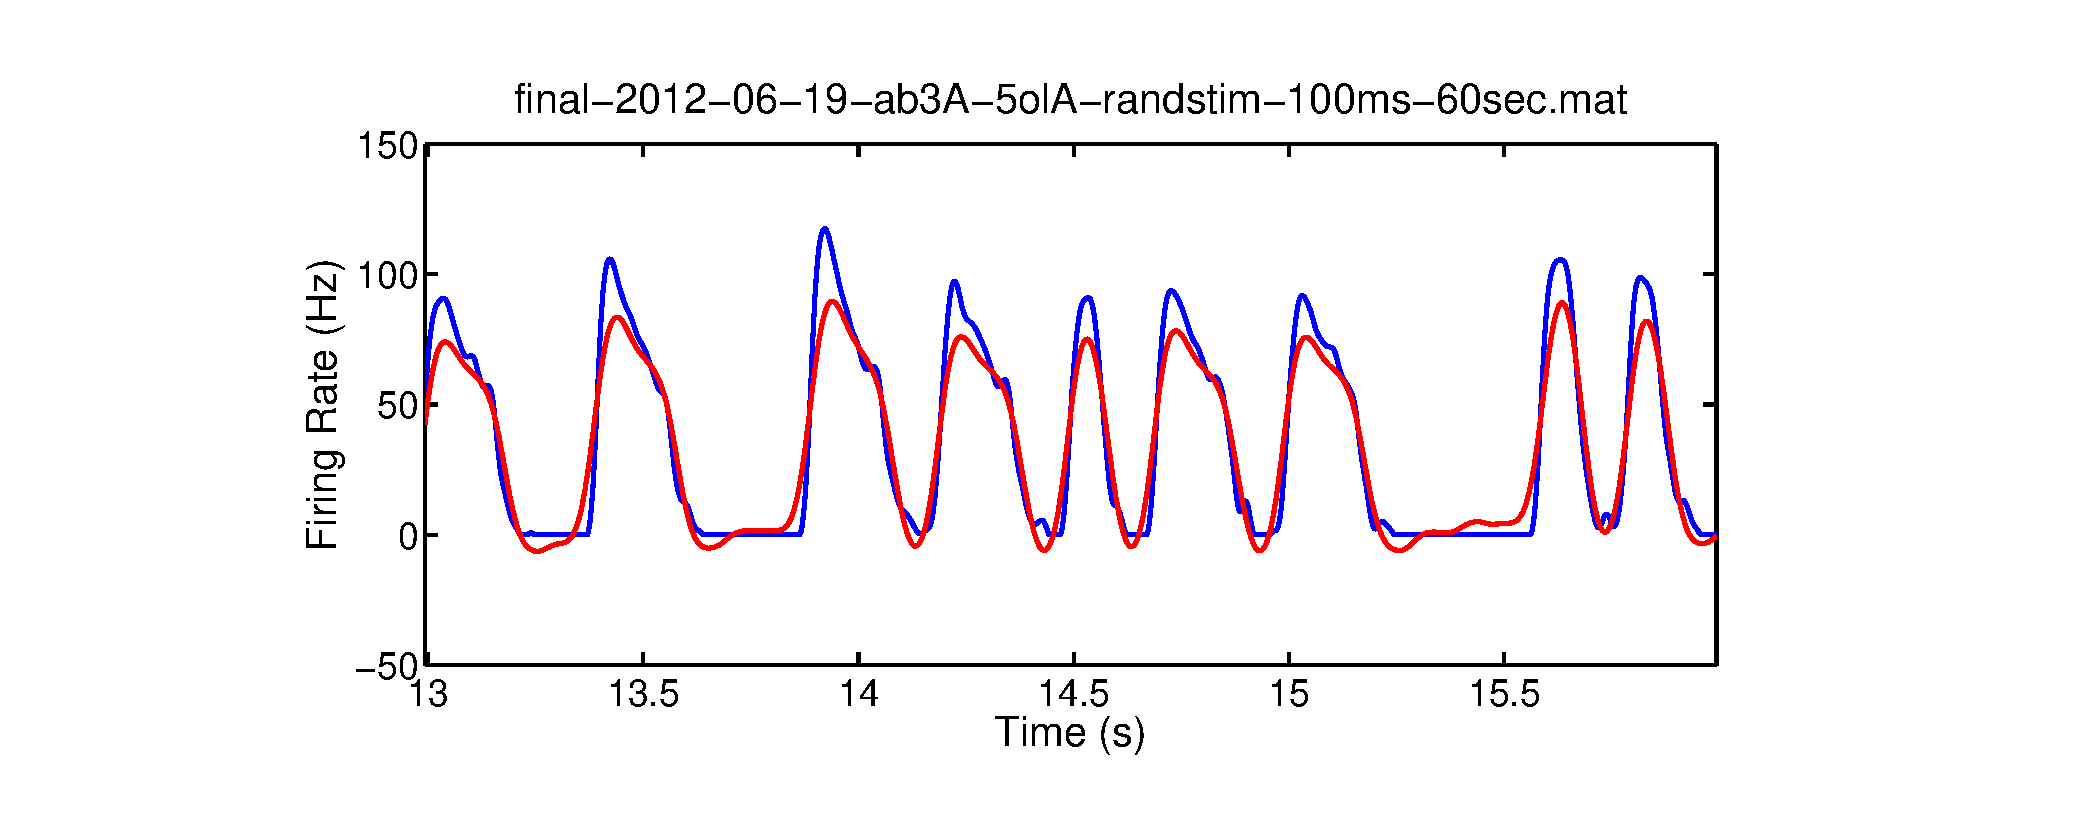
\includegraphics [width=\textwidth]{Analysis_February_19.pdf}
\begin{par}
We now plot the slopes of the prediction to the data for each data set.
\end{par} \vspace{1em}

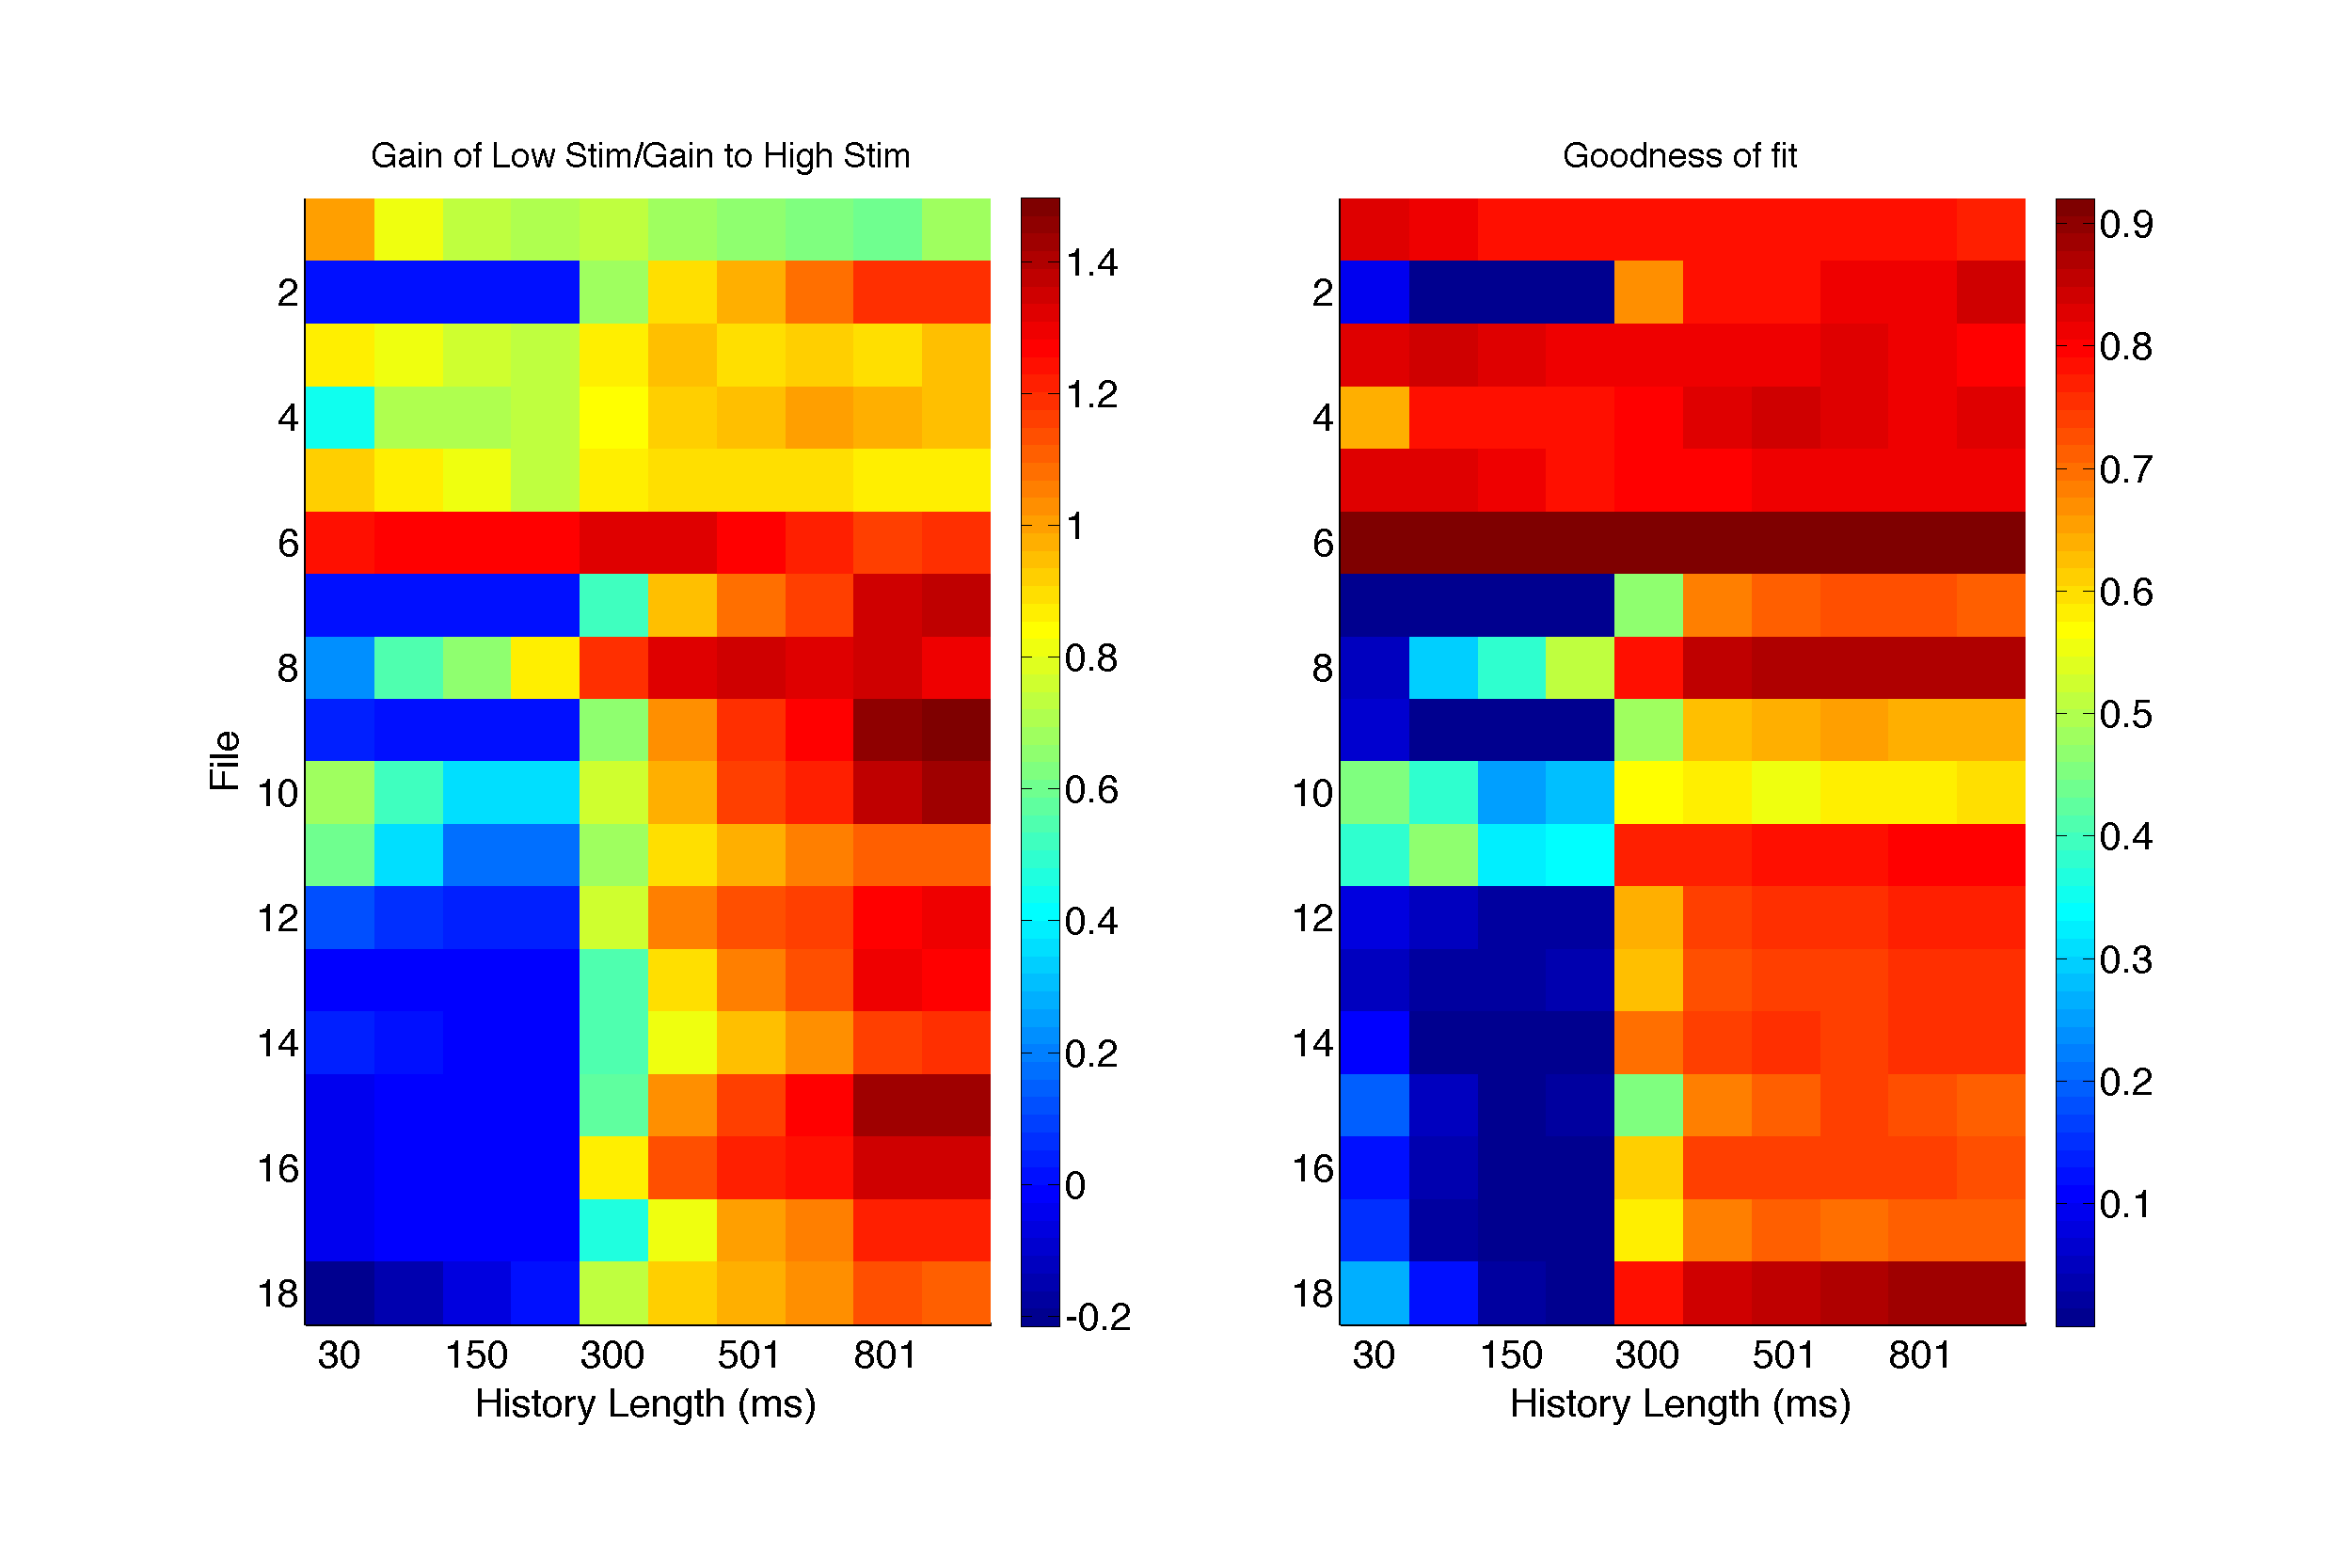
\includegraphics [width=\textwidth]{Analysis_February_20.pdf}


\subsection*{Next Steps}

\begin{enumerate}
\setlength{\itemsep}{-1ex}
   \item Prevent predicted firing rates from going \ensuremath{<} 0 ?
\end{enumerate}


\subsection*{Docs}

\begin{par}
This document was generated by MATLAB's \textit{publish} function. All files needed to generate this document are on a git repository. To clone onto your machine, use:
\end{par} \vspace{1em}
\begin{verbatim}git clone https://srinivasgs@bitbucket.com/srinivasgs/da.git\end{verbatim}
\begin{par}
You will also need a bunch of functions that this depends on, which are also on git. Use
\end{par} \vspace{1em}
\begin{verbatim}git clone https://srinivasgs@bitbucket.com/srinivasgs/core.git\end{verbatim}
\begin{par}
to get these.
\end{par} \vspace{1em}
\begin{par}
Once you have everything, run these commands to generate this document:
\end{par} \vspace{1em}
\begin{verbatim}options = struct('showCode',false,'format','latex','imageFormat',...
'pdf','figureSnapMethod','print','stylesheet','srinivas_latex.xsl');\end{verbatim}
\begin{verbatim}publish2('Analysis_January.m',options);\end{verbatim}



\end{document}
    
